\documentclass[12pt]{article}

% Language setting
% Replace `english' with e.g. `spanish' to change the document language
\usepackage[english]{babel}
\setcounter{section}{-1}

% Set page size and margins
% Replace `letterpaper' with `a4paper' for UK/EU standard size
\usepackage[letterpaper,top=2cm,bottom=2cm,left=3cm,right=3cm,marginparwidth=1.75cm]{geometry}

% Useful packages
\renewcommand{\topfraction}{.85}
\renewcommand{\bottomfraction}{.7}
\renewcommand{\textfraction}{.15}
\renewcommand{\floatpagefraction}{.66}
\renewcommand{\dbltopfraction}{.66}
\renewcommand{\dblfloatpagefraction}{.66}
\setcounter{topnumber}{9}
\setcounter{bottomnumber}{9}
\setcounter{totalnumber}{20}
\setcounter{dbltopnumber}{9}
\usepackage[font=small,labelfont=bf]{caption}
\usepackage{amsmath}
\usepackage{graphicx}
\usepackage{subcaption}
\captionsetup[table]{labelsep=space}
\captionsetup[figure]{labelsep=space}
\usepackage[colorlinks=true, allcolors=blue]{hyperref}
\linespread{1.5}
\setcounter{tocdepth}{4}
\setcounter{secnumdepth}{4}
\setcounter{section}{0}
\newcommand{\myparagraph}[1]{\paragraph{#1}\mbox{}\\}
\title{Part III Systems Biology Project Report\\
\textbf{Modelling Mitochondrial Liver Toxicity With Oxygen and Cell Density Gradients} }

\author{Xingze Xu, University of Cambridge\\
Supervisor: Dr Giovanni Di Veroli, AstraZeneca plc.\\
Deputy supervisor: Dr Aydar Uatay, AstraZeneca plc.\\
Number of words: 4974}
\date{}
\begin{document}
\maketitle
\thispagestyle{empty}
\pagebreak
\thispagestyle{empty}
\section*{Declaration}
Name: Xingze Xu\\
College: Homerton\\
Project title: Modelling Mitochondrial Liver Toxicity With Oxygen and Cell Density Gradients\\
\\
\textit{I understand the University’s definition of plagiarism. I declare that, in accordance with Discipline regulation 6, this dissertation is entirely my own work except where otherwise stated, either in the form of citation of published work, or acknowledgement of the source of any unpublished material.}\\\\
Signature:  \quad\quad\quad\quad\quad\quad\quad\quad\quad\quad\quad\quad      \quad \quad      Date:
\pagebreak


\section*{Summary}
Drug-induced liver injury (DILI) has become a major safety concern in drug development, and various models of DILI have been developed for pre-clinical screening. This thesis presents Systems Model of Drug-Induced Liver Injury (SysDILI), an \textit{in silico} model of human mitochondrial DILI using the holistic approach of systems biology. SysDILI was designed to predict liver toxicity based on mechanism and dose-response of drug while preserving mechanistic and spatiotemporal information for further analysis.\\\\
SysDILI consists of four submodels based on partial or ordinary differential equations, describing dynamics of oxygen, mitochondria, cell density of hepatocytes and drug. The submodels were developed and tested independently before being assembled to study and model their interactions. Instead of artificial liver zonation, continuous spatiotemporal distributions were used throughout.\\\\
While some of the methods and models in SysDILI build on previous research, original advances have also been incorporated in the design of SysDILI. Oxygen transport by haemoglobin was modelled dynamically using a rebalancing process. Coefficients of drug effects were determined by optimisation to handle the complexity of model. Two Hill equation terms were used to capture the combined effects of energy-dependent apoptosis and necrosis.\\\\
After discretisation and numerical simulation of the system in MATLAB, SysDILI successfully predicted the liver toxicity of several known drugs, and the simulated oxygen and cell density gradients also agreed with known results. Further research will aim to add toxicity mechanisms, model longer term DILI and adapt SysDILI to facilitate the \textit{in vitro} model of liver-on-a-chip for practical purpose.


\thispagestyle{empty}
\pagebreak
\thispagestyle{empty}
\tableofcontents
\thispagestyle{empty}
\pagebreak
\section*{List of Abbreviations}
\thispagestyle{empty}
\begin{center}
\begin{tabular}{|c | c|} 
 \hline
 \textbf{Abbreviations} & \textbf{Full meanings} \\
 \hline\hline
 DILI & Drug-Induced Liver Injury  \\ 
 \hline
 MPS & Microphysiological System  \\
 \hline
 ATP & Adenosine Triphosphate\\
 \hline
  OCR & Oxygen Consumption Rate\\
 \hline
  ETC & Electron Transport Chain\\
 \hline
  MMP & Mitochondrial Membrane Potential\\
 \hline
  SysDILI & Systems Model of Drug-Induced Liver Injury\\
 \hline
 ROS & Reactive Oxygen Species\\
 \hline
 Km & Michaelis Constant\\
 \hline
 LDH & Lactate Dehydrogenase\\
 \hline
 ALT & Alanine Transaminase\\
 \hline
 FAST & Fourier Amplitude Sensitivity Testing \\
 \hline
\end{tabular}
\end{center}


\pagebreak
 \clearpage
 \pagenumbering{arabic}
\section{Introduction}
\subsection{Drug-Induced Liver Injury}
The liver - largest internal organ in the human body, is responsible for a variety of functions, such as production of bile, metabolism of glucose and detoxification. It plays a vital role in metabolism of xenobiotics and hence is vulnerable to drug-induced injury \cite{grantDetoxificationPathwaysLiver}. Drug-induced liver injury (DILI) can occur via many mechanisms, the most prominent ones being mitochondrial dysfunction, bile acid-induced apoptosis and oxidative stress by reactive oxygen species (ROS) or reactive nitrogen species \cite{jaeschkeMechanismsHepatotoxicity2002}.\\\\
DILI tends to be non-uniformly spatially distributed across the liver. For example,  overdoses of acetaminophen have been reportedto damage the region surrounding the central vein \cite{anundiZonationAcetaminophenMetabolism1993a}. Such distribution can be explained by the non-homogeneous stucture of the liver: the most basic functional unit, liver acinus, is characterized by zonation \cite{mancoLiverZonation2021}. It is commonly accepted that each acinus is divided into three zones from portal triad to central vein, periportal (zone 1), intermediate (zone 2) and perivenous (zone 3), as shown in Figure \ref{fig:0} \cite{kietzmannMetabolicZonationLiver2017a,godoyRecentAdvances2D2013}. Liver zonation is eflected in two interacting aspects: (1) gradients of substances, including oxygen, nutrients, xenobiotics, morphogens, hormones and enzymes; (2) gradients of rates in metabolic and regulatory pathways, such as bile acid production and detoxification mostly happening in zone 3 \cite{kietzmannMetabolicZonationLiver2017a}. 
Therefore, liver zonation plays a crucial role in the study of DILI.\\\\
\begin{figure}[h!]
\centering
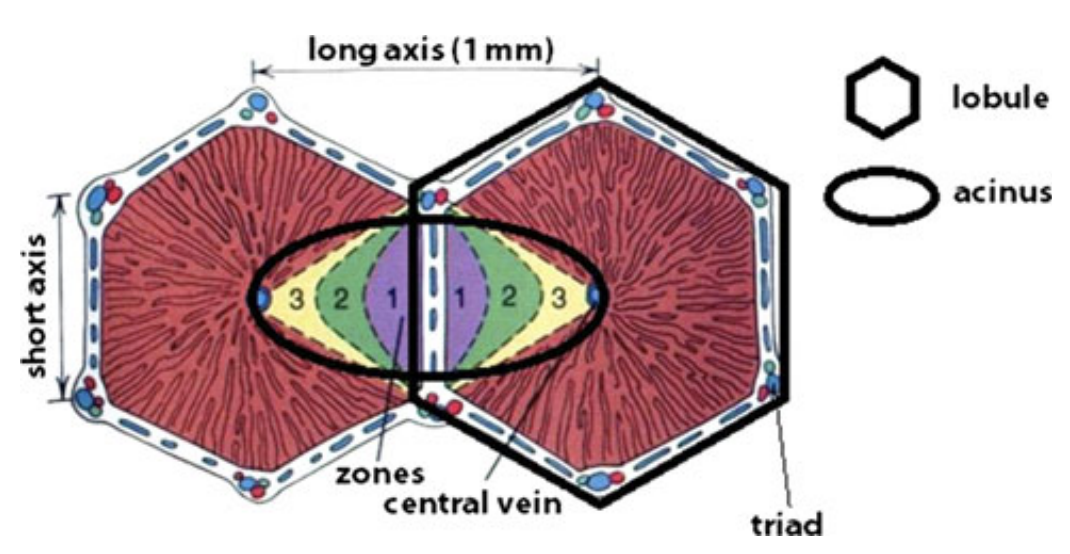
\includegraphics[width = 8cm, height = 4cm]{acinus.png}
\caption{Structure of liver acinus and distribution of the three zones. Diagram from Godoy et al. \cite{godoyRecentAdvances2D2013}}.
\label{fig:0}
\end{figure}DILI has become a major safety concern in drug development, causing 22 percent of clinical trial terminations and 32 percent of market withdrawals \cite{watkinsDrugSafetySciences2011a}. Even when signs of abnormalities in liver are reported during clinical trials, the regulators might demand additional clinical trials to assess liver safety, which can substantially increase costs of drug development programs.
\subsection{Previous Work on Modelling DILI}
Due to its importance in drug development, various models of DILI have been developed for pre-clinical screening.
\subsubsection{\textit{In Vitro} Model}
Apart from animal models, recent years have seen rapid development of more sophisticated 3D \textit{in vitro} cell culture models, including spheroid, organoid, scaffold, organ-on-a-chip and 3D bioprinting \cite{fangThreeDimensionalCellCultures}.\\\\
The spheroid culture system has been commonly used to investigate hepatotoxicity \cite{leedaleSilicoguidedOptimisationOxygen2019}. As opposed to the traditional 2D monolayer cell culture, spheroid culture provides a simple solution to capture spatial gradients of oxygen, drug, nutrients or signalling molecules, because cells in central and peripheral parts of the spheroid have different exposure to the culture medium \cite{fangThreeDimensionalCellCultures}.\\\\Organ-on-a-chip, or microphysiological system (MPS) is another common but more advanced 3D \textit{in vitro} culture model. It utilizes microfluidic devices with specific design and electronic control to simulate the microenvironment and important physiological features of organs. MPS for liver has been relatively well developed, and it is widely used in the pharmaceutical industry for pre-clinical screening. Figure \ref{fig:2} shows a typical design of the device \cite{peelIntroducingAutomatedHigh2019a}. While it has advantages, MPS also has some limitations – it is complicated and time-consuming, taking up to 7 days to set up before drug intake \cite{peelIntroducingAutomatedHigh2019a}.
Despite efforts to increase the throughput, it remains challenging to detect and interpret the trial results of liver MPS.

\begin{figure}[h!]
\centering
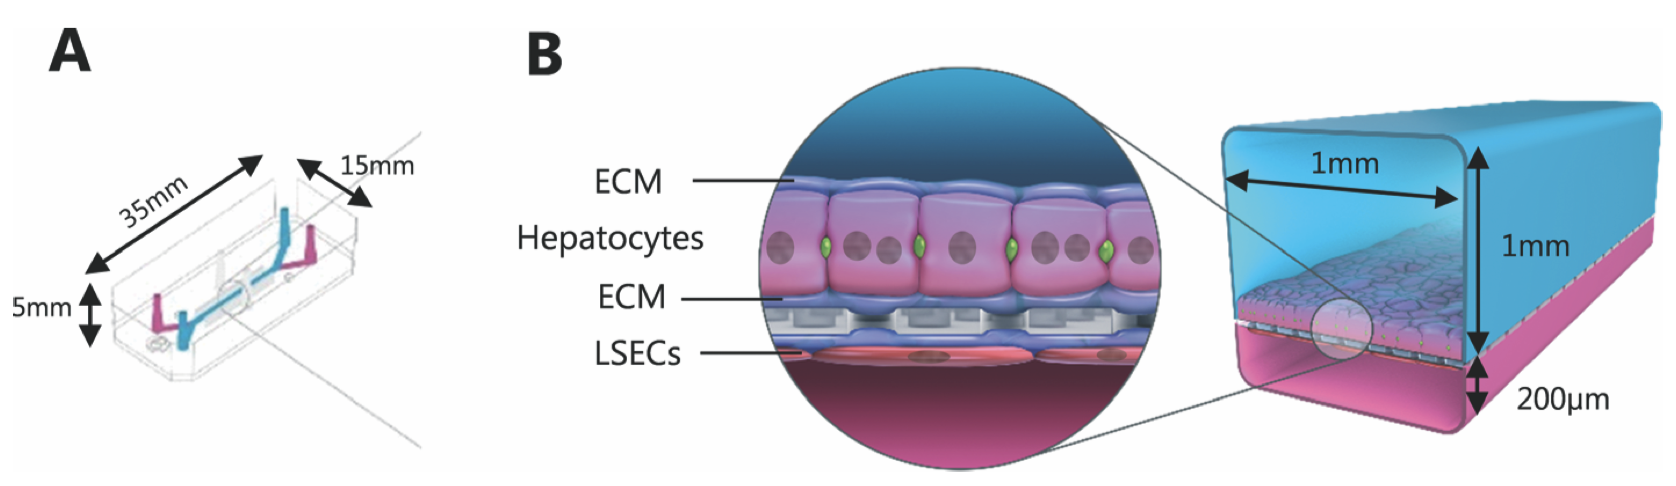
\includegraphics[width = 14cm, height = 4cm]{mps.png}
\caption{Deisgn of a liver MPS. (A) Dimensions of the MPS; (B) two cell types in the MPS: hepatocypte and liver sinusoidal endothelial cell (LSEC). The interface is coated with extracellular matrix (ECM). Culture media are flown across the cell layers. Diagram from Peel et al. \cite{peelIntroducingAutomatedHigh2019a}}.
\label{fig:2}
\end{figure}

\subsubsection{\textit{In Silico} Model}
With the operational complexity of \textit{in vitro} models in mind, researchers have developed \textit{in silico} liver models to simulate \textit{in vitro} liver models. Multiphysics simlution software such as COMSOL has been used to investigate the drug distribution in spheroid culture and guide the design of oxygen suppply of liver MPS \cite{leedaleMultiscaleModellingDrug2020,lee-montielControlOxygenTension2017}.\\\\There are also more complicated \textit{in silico} models aiming to directly model DILI in human. DILIsym\textsuperscript{\textregistered} by Simulations Plus Inc. is a Quantitative Systems Toxicology software for human DILI that consists of a dozen interacting sub-modules, as shown in Figure \ref{fig:3} \cite{DILIsymDruginducedLiver}. As opposed to the multiphyics simulations based on partial differential equations (PDE), DILIsym\textsuperscript{\textregistered} is partitioned into the three liver zones each with its set of ordinary differential equations (ODE).

\begin{figure}[h!]
\centering
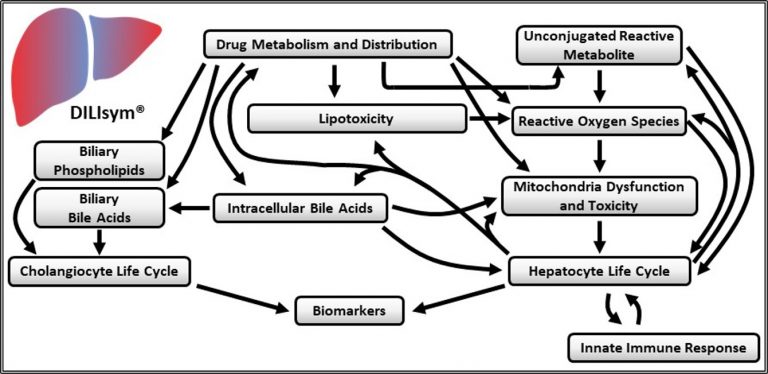
\includegraphics[width = 14cm, height = 7cm]{dilisym.jpeg}
\caption{Schematic diagram of DILIsym\textsuperscript{\textregistered}. The boxes represent submodels that can be inspected alone. An arrow indicates that variables in one submodel affect the rate of one or more processes in another submodel. For example, high concentration of ROS activates apoptosis in hepatocyte life cycle \cite{finkelSignalTransductionMitochondrial2012}. Diagram from DILIsym\textsuperscript{\textregistered} website \cite{DILIsymDruginducedLiver}}.
\label{fig:3}
\end{figure}

\subsection{Systems Model of Drug-Induced Liver Injury (SysDILI)}
Systems Model of Drug-Induced Liver Injury (SysDILI) is the \textit{in Silico} DILI model presented in this thesis. Important features of SysDILI are summarised below.
\begin{itemize}
    \item \textbf{Modular}: as in Figure \ref{fig:1}, SysDILI consists of four interacting submodels, in the same spirit as the aforementioned DILIsym\textsuperscript{\textregistered}. Each submodel was developed and tested independently, so they can be freely assembled. It is also convenient to add new submodels such as glycolysis model without changing the existing ones.
    \item \textbf{Continuous Spatiotemporal Gradients}: the gradients in each submodel are spatially continuous with no artificial zonation, in the same spirit as the aforementioned multiphysics simulations. Also, the temporal dynamics for each gradient was modelled, not just the equilibrium states.
     \item \textbf{Continuum of Domains}: no individual hepatocyte or blood cell in SysDILI. Each domain was modelled as continuum.
    \item \textbf{Mitochondrial Toxicity}: out of the various DILI mechanisms mentioned above, SysDILI currently focuses on mitochondrial toxicity (reasons outlined in Discussion section).
    \item \textbf{Dry Lab}: no experiments have been conducted so far. SysDILI was constructed entirely from published data.
    
    \item \textbf{Flexible and Customisable}: SysDILI currently models a sinusoid functional unit of human liver, but it can be readily adapted to MPS by changing the shapes of domains and the boundary conditions, because all the model parameters have been estimated and no gradient data was enforced during model construction.
    \item \textbf{Aim to Be Mechanistic}: the entire process was modelled whenever possible, including the changes in intermediate variables and temporal dynamics. Black box models were only used when mechanistic modelling requires extensive amount of insights or experimental data.
    
\end{itemize}
\begin{figure}[h!]
\centering
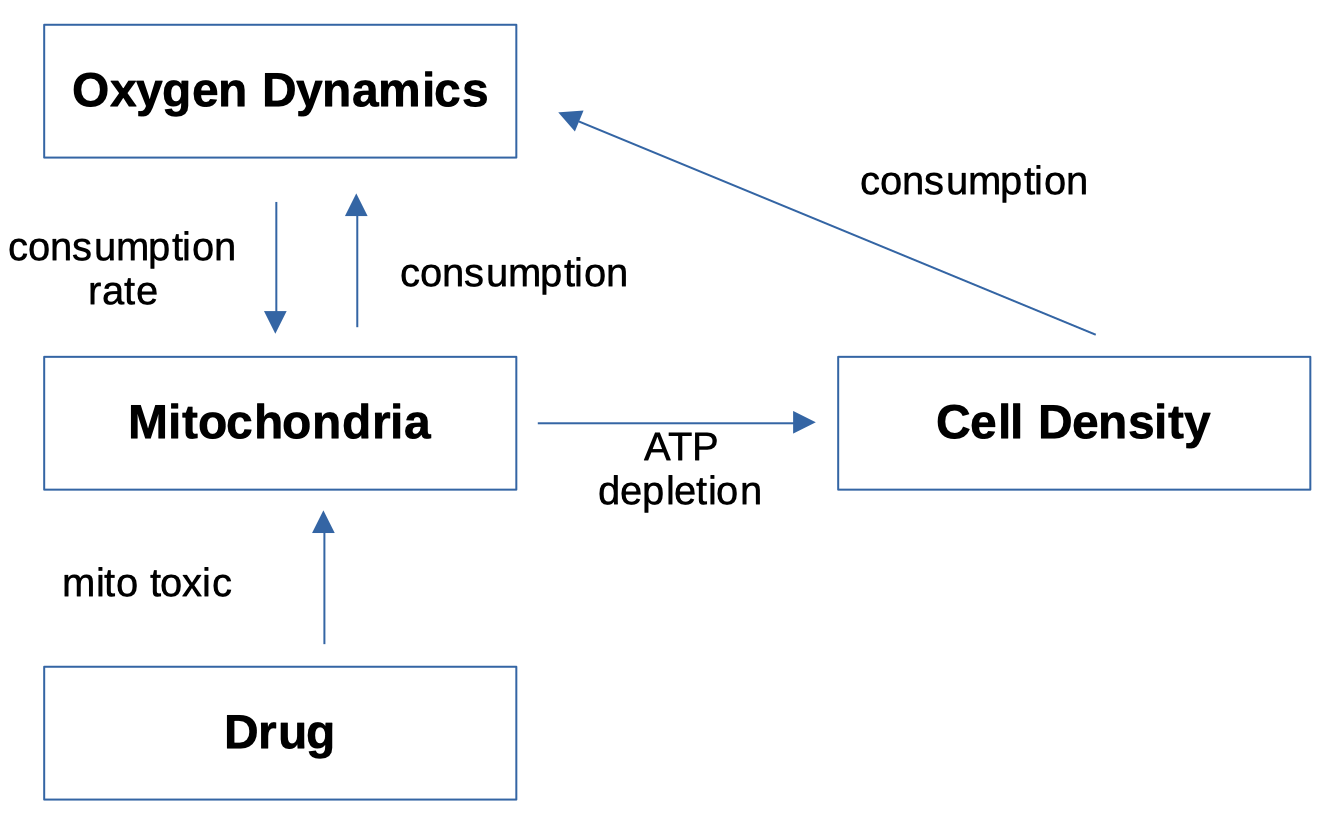
\includegraphics[width = 9cm, height = 6.5cm]{overall.png}
\caption{Schematic diagram of SysDILI. The diagram shows the submodels of SysDILI and their interactions. Drug affects mitochondria by its toxicity, which causes ATP depletion and cell death. Oxygen consumed by mitochondria is proportional to cell density, and oxygen concentration conversely affects the state of mitochondrial activities.}
\label{fig:1}
\end{figure}
The SysDILI model aims primarily to predict DILI based on mechanism and dose-response curve of an unknown drug. In addition to assessing hepatotoxicity, SysDILI was also designed to preserve as much mechanistic and spatiotemporal information as possible. The extra information can be compared against physiological data for validation and might even reveal extra insights. With the flexibility mentioned above, SysDILI can be used to guide the design of MPS and interpret the results.
\section{Results}
\subsection{SysDILI Model}
As said in Introduction section, SysDILI consists of four submodels, describing dynamics of oxygen, mitochondria, cell density of hepatocytes and drug, as in Figure \ref{fig:1}. These four submodels were selected because they play crucial roles in mitochondrial DILI and interact with each other. Drug inhibits mitochondrial function, which causes ATP depletion and eventually cell death. Mitochondria consumes oxygen in proportional to cell density, while oxygen concentration conversely affects the state of mitochondrial respiration.
\subsubsection{Oxygen Submodel}
The domain setup of SysDILI is defined in the Oxygen Submodel. In this thesis, a sinusoid functional unit of human liver was modelled, with a hepatic sinusoid extending from portal triad to central vein, surrounded by one layer of hepatocytes.\\\\Since liver sinusoid is a special type of capillary, a design similar to Krogh model of oxygen transport in capillary was used, as shown in Figure \ref{fig:oxy} \cite{goldmanTheoreticalModelsMicrovascular2008}. 3D cylindrical coordinate with rotational symmetry about the axial direction was used, and the schematic diagram shows radial and axial directions. There are three domains: sinusoid, hepatocytes and their interface. Oxygen supplied from blood flowing through the left end of sinusoid falls into two categories, plasma oxygen and haemoglobin oxygen. After plasma oxygen diffuses across the interface, it gets consumed by hepatocytes. 
\begin{figure}[h!]
\centering
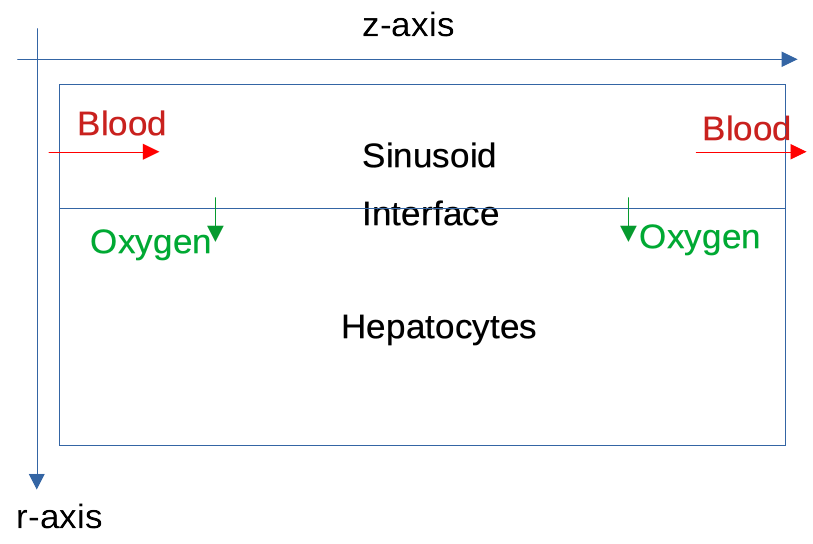
\includegraphics[width = 8cm, height = 6cm]{oxy_sketch.png}
\caption{Schematic diagram of SysDILI domain setup and Oxygen Submodel. This setup is for the simulation of human liver sinusoid unit. 3D cylindrical coordinate system is centred at the top-left corner with z-axis horizontal. Blood with oxygen flows through the sinusoid, and some of the oxygen diffuses across the interface and gets consumed by hepatocytes.}
\label{fig:oxy}
\end{figure}
\myparagraph{Model Structure}
The submodel is defined by the 5 PDEs listed below.
\begin{itemize}
    \item \textbf{Plasma Oxygen}: convection-diffusion equation was used, because oxygen dissolved in plasma diffuses while being carried by flood flow. \[\frac{\partial P}{\partial t}=D_1*\nabla^2P-\boldsymbol{v}\cdot \nabla P=D_1*(\frac{\partial^2 P}{\partial r^2}+\frac{\partial^2 P}{\partial z^2}+\frac{1}{r}*\frac{\partial P}{\partial r})-v*\frac{\partial P}{\partial z}\]
\item \textbf{Haemoglobin Oxygen}: convection equation was used, because oxygen does not diffuse when bound to haemoglobin. \[\frac{\partial H}{\partial t}=-\boldsymbol{v}\cdot \nabla H=-v*\frac{\partial H}{\partial z}\]
\item \textbf{Oxygen Equilibrium}: Hill equation was used to describe the haemoglobin-oxygen dissociation curve \cite{leowConfigurationHemoglobinOxygen2007}. This only holds true when haemoglobin and plasma oxygen are in equilibrium (details in Section \ref{section:haemo}).
\[H=H_{max}*\frac{{P}^{h}}{{P}^{h}+{K_A}^{h}}
\]
\item \textbf{Oxygen in Hepatocytes}: diffusion-reaction was used, because there is no more convection of oxygen by blood flow. Michaelis-Menten kinetics was used for oxygen consumption by hepatocytes \cite{leedaleSilicoguidedOptimisationOxygen2019}. \[\frac{\partial O_2}{\partial t}=D_2*\nabla^2O_2-R(O_2)=D_2*(\frac{\partial^2 O_2}{\partial r^2}+\frac{\partial^2 O_2}{\partial z^2}+\frac{1}{r}*\frac{\partial O_2}{\partial r})-\frac{O_2*v_{max}}{O_2+k_m}\]
\item\textbf{Oxygen at the Interface}: equal-flux condition was used, because mass is conserved when oxygen moves across the interface \cite{leedaleSilicoguidedOptimisationOxygen2019}.\[D_1*\frac{\partial P}{\partial r}=D_2*\frac{\partial O_2}{\partial r}\]
\end{itemize}
 $P$, $H$ and $O_2$ are oxygen concentrations in hepatocyte, dissolved in plasma and bound to haemoglobin, respectively. $D_1$ and $D_2$ are oxygen diffusion coefficients in plasma and hepatocytes, respectively. $v$ is sinusoid blood flow velocity assumed to be fixed in this model. $v_{max}$ and $k_m$ are constants for Michaelis-Menten kinetics of oxygen consumption in hepatocytes.\\\\The PDE system was discretised both in time ($\Delta t=4.5*10^{-3}s$) and space ($\Delta x=2 \mu m$) before being simulated numerically. Details of the numerical algorithm, the boundary conditions and the choice of constants are elaborated in Methods section.
\myparagraph{Haemoglobin Oxygen Release}\label{section:haemo}
Oxygen bound to haemoglobin is released when the plasma oxygen concentration decreases due to diffusion, moving down the haemoglobin-oxygen dissociation curve. The rate constant of oxyhemoglobin dissociation suggests that the process is much faster than oxygen diffusion in plasma \cite{olsonMeasurementRateConstants2003}. Therefore, in the discretised numerical algorithm it was assumed that haemoglobin releases oxygen and the equilibrium is instantaneously reached at the end of each time step. This process is termed rebalancing, as shown in Figure \ref{fig:hemo}, where $P_n$ and $\Bar{P}_n$ stand for plasma oxygen concentrations at $n$-th time step before and after rebalancing, respectively. Similarly, $H_n$ and $\Bar{H}_n$ represent concentrations of oxygen bound to haemoglobin at $n$-th time step before and after rebalancing, respectively. 
\begin{figure}[h!]
\centering
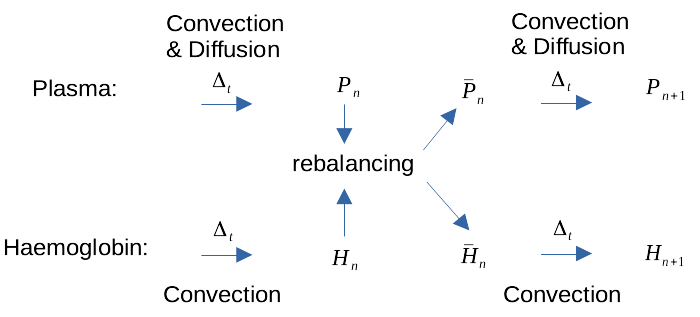
\includegraphics[width = 12cm, height = 5.4cm]{hemo_sketch.png}
\caption{Schematic diagram of oxygen rebalancing in sinusoid. Haemoglobin oxygen and plasma oxygen are updated in parallel in each time step by different iteration matrices, but they get rebalanced to reach equilibrium at the end of time step, under the assumption that this process is relatively fast.}
\label{fig:hemo}
\end{figure}
\begin{equation}
\begin{aligned}
& \Bar{P}_n+\Bar{H}_n=P_n+H_n \\
& \Bar{H}_n=H_{max}*\frac{{\Bar{P}_n}^{h}}{{\Bar{P}_n}^{h}+{K_A}^{h}}\\
\end{aligned}
\label{eqn:reba}
\end{equation}
Equation \ref{eqn:reba} shows the exact procedure of rebalancing, during which $\Bar{H}_n$ and $\Bar{P}_n$ are solved from known $H_n$ and $P_n$. Haemoglobin-oxygen dissociation curve is described by Hill equation, with the Hill coefficient h=2.73 and $K_A=26$ mmHg, concentration of plasma oxygen with half of haemoglobin saturated \cite{valabregueRelationCerebralBlood2003}. $H_{max}=6865.67$ mmHg is the total concentration of haemoglobin oxygen when haemoglobin is 100\% saturated \cite{valabregueRelationCerebralBlood2003}.
\myparagraph{Validation}


\begin{figure}[ht]
\begin{subfigure}{0.5\textwidth}
\centering
    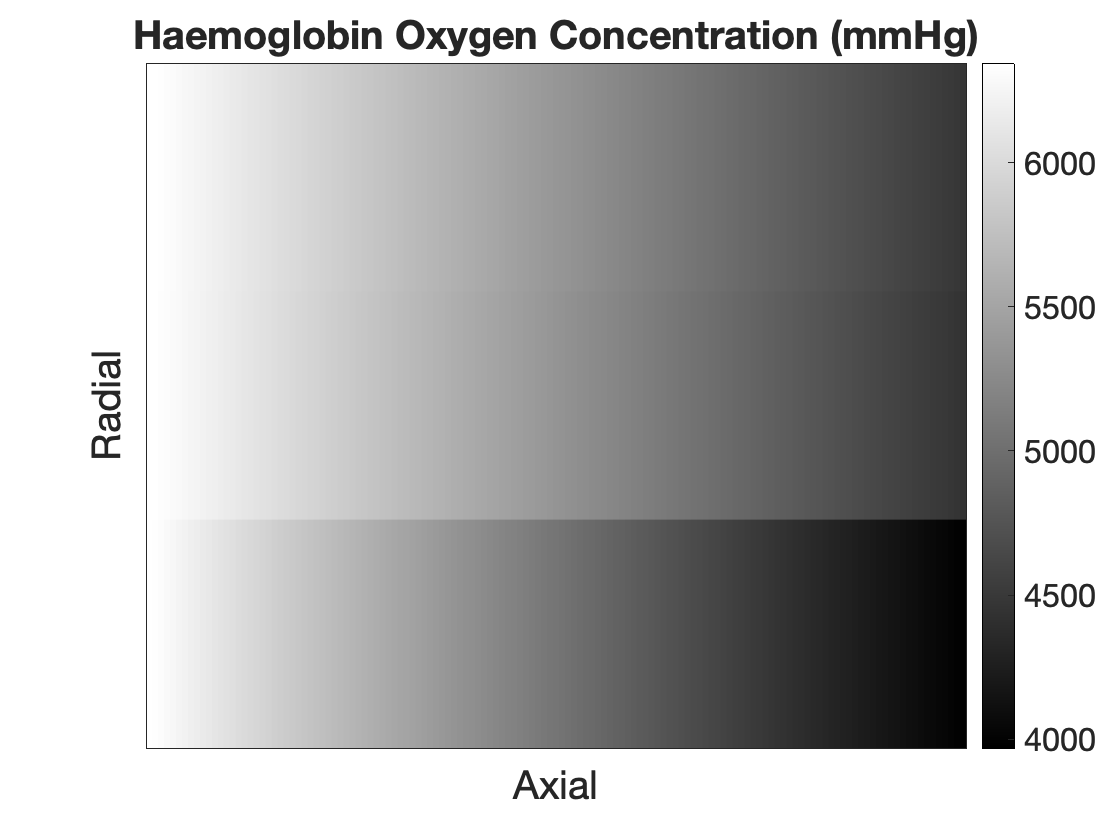
\includegraphics[width=\linewidth]{haemo.png} 
    \caption{}
    \label{fig:oxy_1}
\end{subfigure}
\hfill
\begin{subfigure}{0.5\textwidth}
\centering
    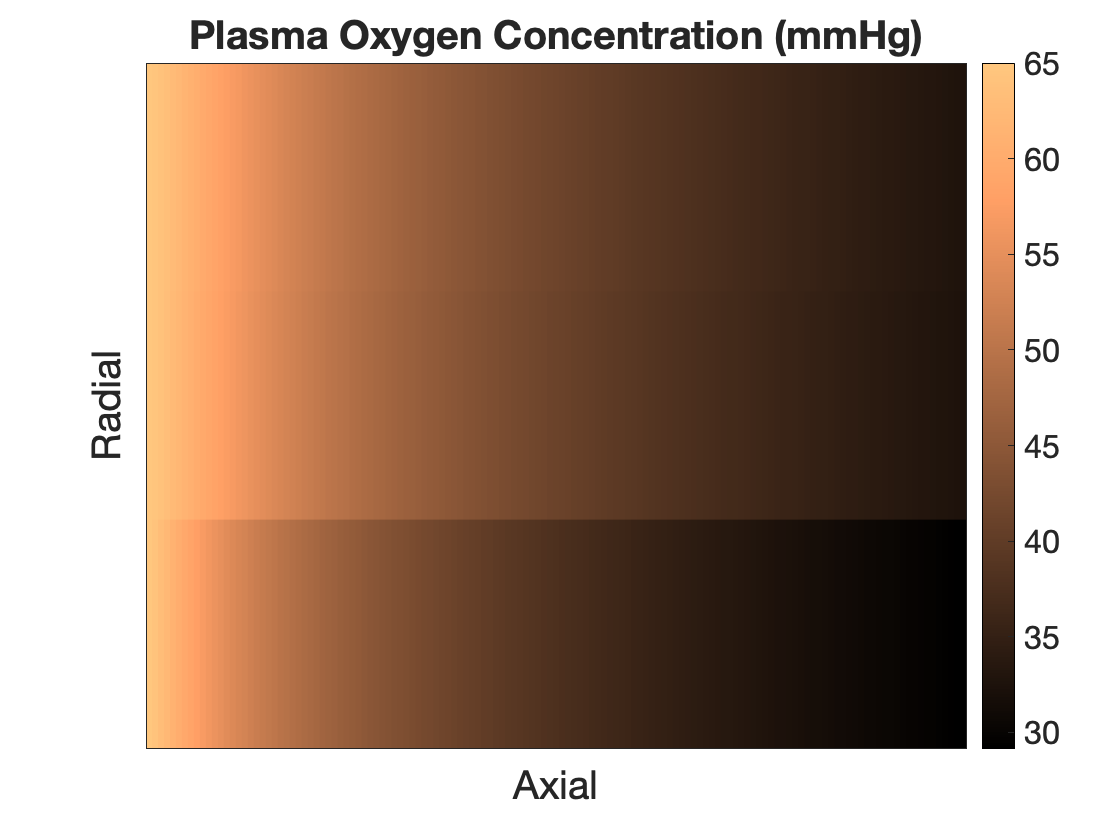
\includegraphics[width=\linewidth]{plasma.png} 
    \caption{}
   \label{fig:oxy_2}
\end{subfigure}
\hfill
\begin{subfigure}{0.5\textwidth}
\centering
    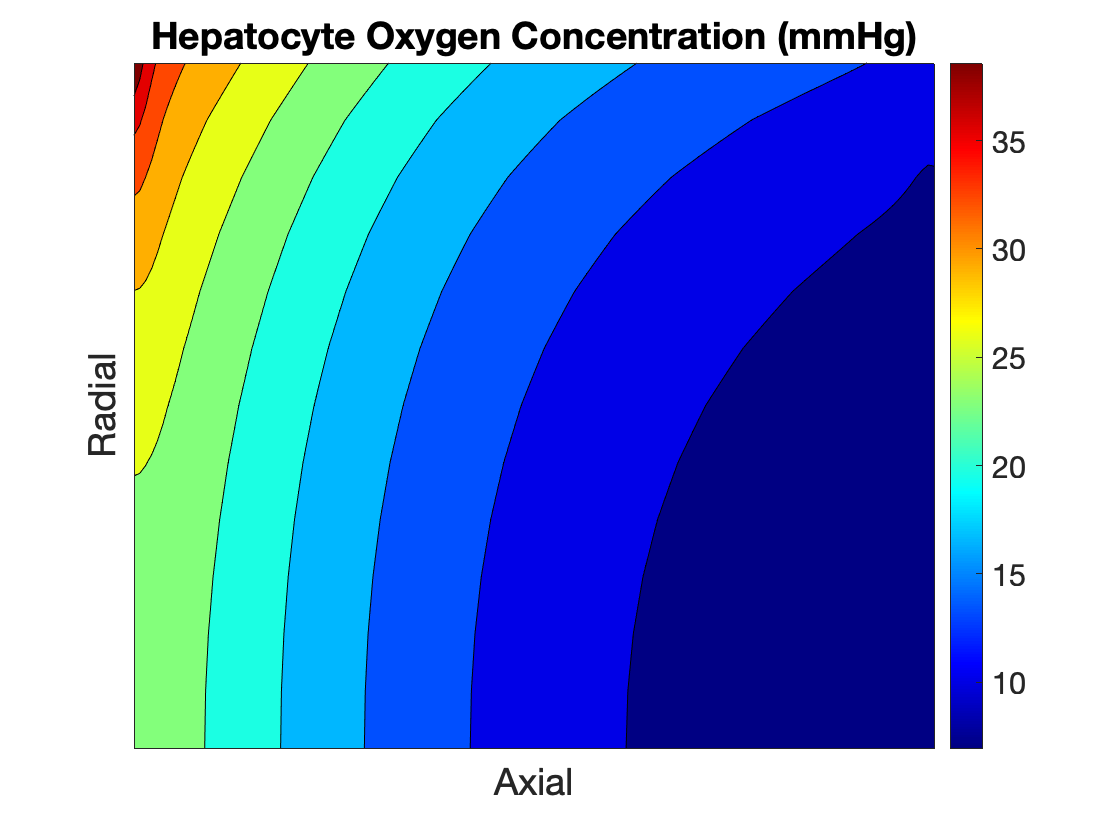
\includegraphics[width=\linewidth]{hepa.png} 
    \caption{}
    \label{fig:oxy_3}
\end{subfigure}
\hfill
\begin{subfigure}{0.5\textwidth}
\centering
    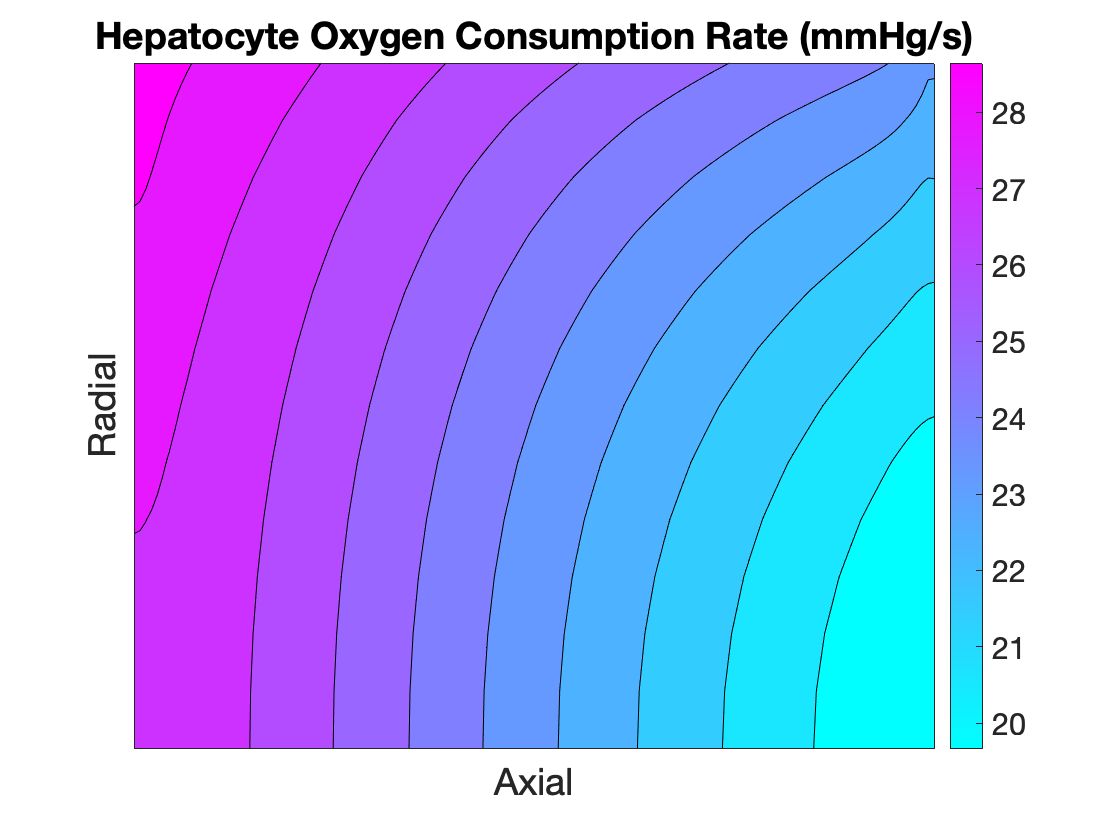
\includegraphics[width=\linewidth]{ocr.png} 
    \caption{}
    \label{fig:oxy_4}
\end{subfigure}
\hfill
  \caption{Simulation outcomes of Oxygen Submodel. (a) Haemoglobin oxygen concentration; (b) plasma oxygen concentration; (c) hepatocyte oxygen concentration; (d) hepatocyte oxygen consumption rate. The axes and layout in all plots are the same as those illustrated in Figure \ref{fig:oxy}. Gradients of oxygen and oxygen consumption rate (OCR) were successfully simulated. (a) and (b), (c) and (d) have similar gradient patterns as expected.}
  \label{fig:quad} 
\end{figure}
\begin{figure}[h!]
\centering
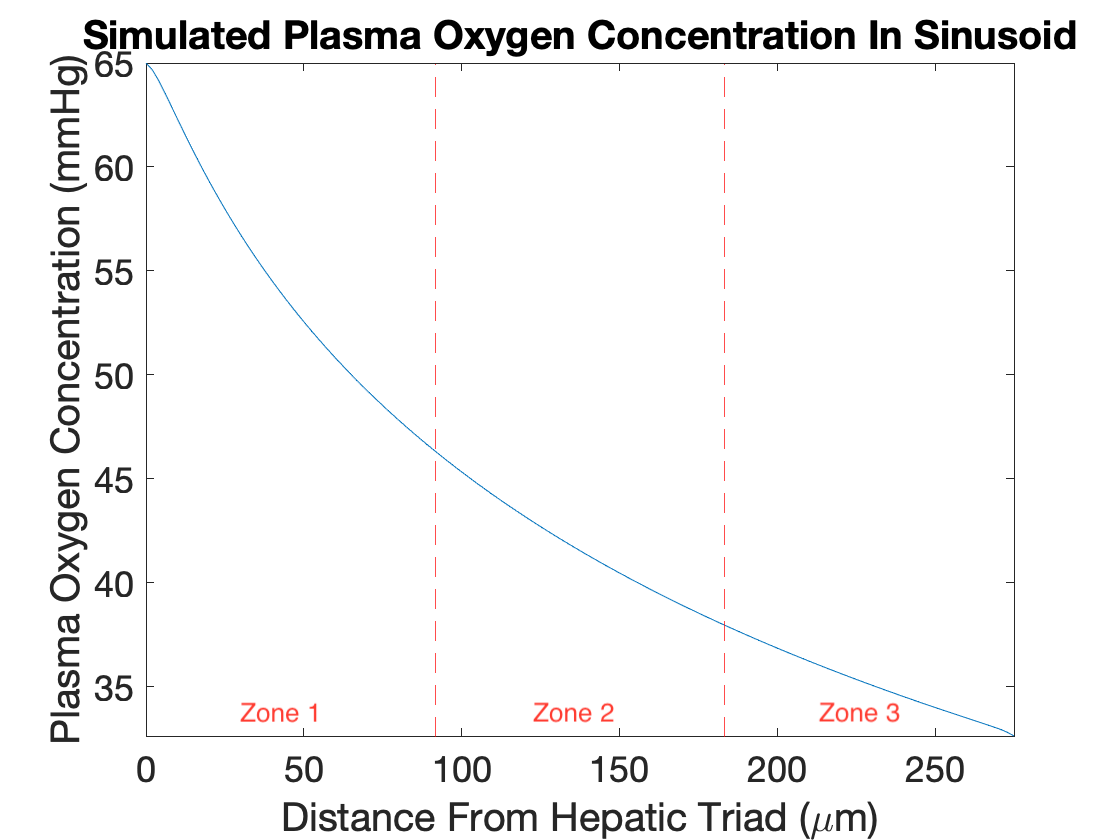
\includegraphics[width = 10cm, height = 9cm]{oxy_vali.png}
\caption{Simulated plasma oxygen concentration along the central axis of sinusoid. The oxygen input at the entrance of zone 1 was fixed to 65 mmHg as in the human liver, and then desired result of approximately 35 mmHg was observed in the simulation outcome of zone 3. }
\label{fig:oxy_vali}
\end{figure}
Figure \ref{fig:quad} shows output of different domains from Oxygen Submodel. Gradients of oxygen concentration and oxygen consumption rate (OCR) were effectively created \textit{in silico}. Figure \ref{fig:oxy_1} and Figure \ref{fig:oxy_2} show similar gradients because plasma oxygen and haemoglobin are in equilibrium, described by Hill equation. Figure \ref{fig:oxy_3} and Figure \ref{fig:oxy_4} show similar gradients because OCR versus oxygen concentration follows Michaelis-Menten kinetics and $v_{max}$ is not reached. Both results were excepted and hence validate the simulation outcomes of Oxygen Submodel.\\\\
In human hepatic sinusoid, the plasma oxygen concentration is approximately 65 mmHg in zone 1 and 35 mmHg in zone 3 \cite{jungermannOxygenModulatorMetabolic2000}. By fixing the boundary condition of plasma oxygen concentration at entry of zone 1 to be 65 mmHg, the simulated outcome at exit of zone 3 is close to 35 mmHg, as shown in Figure \ref{fig:oxy_vali}.
\myparagraph{Sensitivity Analysis} \label{section:sens}
\begin{figure}[h!]
\centering
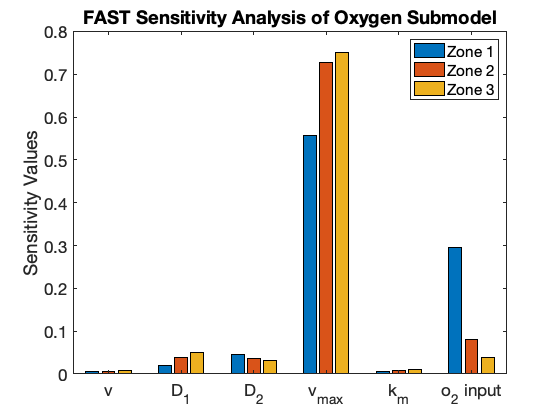
\includegraphics[width = 11cm, height = 9cm]{sens.png}
\caption{FAST Sensitivity analysis of average oxygen concentration in each zone to the parameters of Oxygen Submodel. $O_2$ input represents the Dirichlet boundary condition at the entrance of sinusoid. Range of each parameter was centred at the value picked for the model, with upper and lower bounds one order of magnitude apart. The results show that oxygen concentration is the most sensitive to $v_{max}$, especially in zone 3.}
\label{fig:sens}
\end{figure}
Global sensitivity analysis of the average oxygen concentration in each zone to the parameters was carried out using Fourier amplitude sensitivity testing (FAST), and the results are shown in Figure \ref{fig:sens}. In all zones, oxygen concentration is the most sensitive to the change in $v_{max}$, the maximum OCR. Compared with other zones, oxygen concentration in zone 1 is more sensitive to oxygen input as expected, which validates the results.\\\\
The sensitivity analysis confirms the significance of Oxygen Submodel, because $v_{max}$ will change from a parameter to a variable after Oxygen Submodel is assembled with Mitochondria or Density Submodel, while all other parameters are fixed to values from physiological data. When drug inhibits mitochondrial activities, maximum OCR of the cell will be reduced (see Section \ref{section:mito}), resulting in significant change in oxygen concentration that would not have been taken into account if mitochondria was modelled alone \cite{y.yangMITOsymMechanisticMathematical2015}.
\subsubsection{Mitochondria Submodel} \label{section:mito}
The submodel was adapted and simplified from MITOsym\textsuperscript{\textregistered} introduced in Yang et al., a mechanistic hepatocyte model of bioenergetics  \cite{y.yangMITOsymMechanisticMathematical2015}. Three different toxicity mechanisms are supported: electron transport chain (ETC) inhibitor, uncoupler and ATPase inhibitor.
\myparagraph{Model Structure}
\begin{equation}
\label{eq:1}
\begin{aligned}
&\frac{pyr2ox}{pyr2ox_{basal}}=\frac{k_1^{k_2}+\phi_{basal}^{k_2}}{k_1^{k_2}+\phi^{k_2}}*\frac{k_3^{k_4}+OX_{basal}^{k_4}}{k_3^{k_4}+OX^{k_4}}\\
&\frac{dOX}{dt}=-ETCF+pyr2ox\\
& OCR=q_1*ETCF\\
& ETCF=\frac{1}{q_1}*\frac{O_2*v_{max}}{O_2+k_m}*\frac{OX}{OX_{basal}}*drug_{etc}\\
&\frac{d\phi}{dt}=q_2*ETCF-q_3*ATPF-drug_{uncoupler} \\
&ATPF=\frac{\phi*k_5}{\phi+q_4}*\frac{2*ATPC_{basal}}{ATPC_{basal}+ATPC}*drug_{ATPase}\\
&\frac{dATPC}{dt}=q_5*ATPF-q_6*ATPC 
\end{aligned} \end{equation}
\begin{equation}
\label{eq:2}
\begin{aligned}
& drug_{etc}=\frac{{km}_1}{{km}_1+C}\\
& drug_{uncoupler}=\phi*\frac{k_6*C}{{km}_2+C}\\& drug_{ATPase}=\frac{{km}_3}{{km}_3+C}\end{aligned} \end{equation}
\begin{table}
\begin{tabular}{|c | c|} 
 \hline
 \textbf{Variables} & \textbf{Meanings} \\
 \hline\hline
 pyr2ox & Rate of pyruvate as oxidative substrate in mitochondria \\ 
 \hline
   OX & Mitochondrial oxidative substrate\\
 \hline
  ETCF & Rate of oxidative substrate used for ETC activity, target of \textbf{ETC inhibitor}\\
 \hline
 OCR & Oxygen Consumption Rate\\
 \hline
 $O_2$ & Oxygen concentration \\
  \hline

 $\phi$ & Mitochondrial Membrane Potential, target of \textbf{Uncoupler}\\
 \hline
 ATPF & Rate of mitochondria ATP production, target of \textbf{ATPase inhibitor}\\
 \hline
 ATPC & Cellular ATP\\
 \hline
\end{tabular}
\caption{Meanings of variables in Equation \ref{eq:1}}
\label{Tab:1}
\end{table}\\\\Equation \ref{eq:1} defines the structure of the submodel, with the meanings of all variables listed in Table \ref{Tab:1}. Equation \ref{eq:2} defines the effect of drug with each toxicity mechanism, where C is the concentration of each drug respectively.
\begin{figure}[h!]
\centering
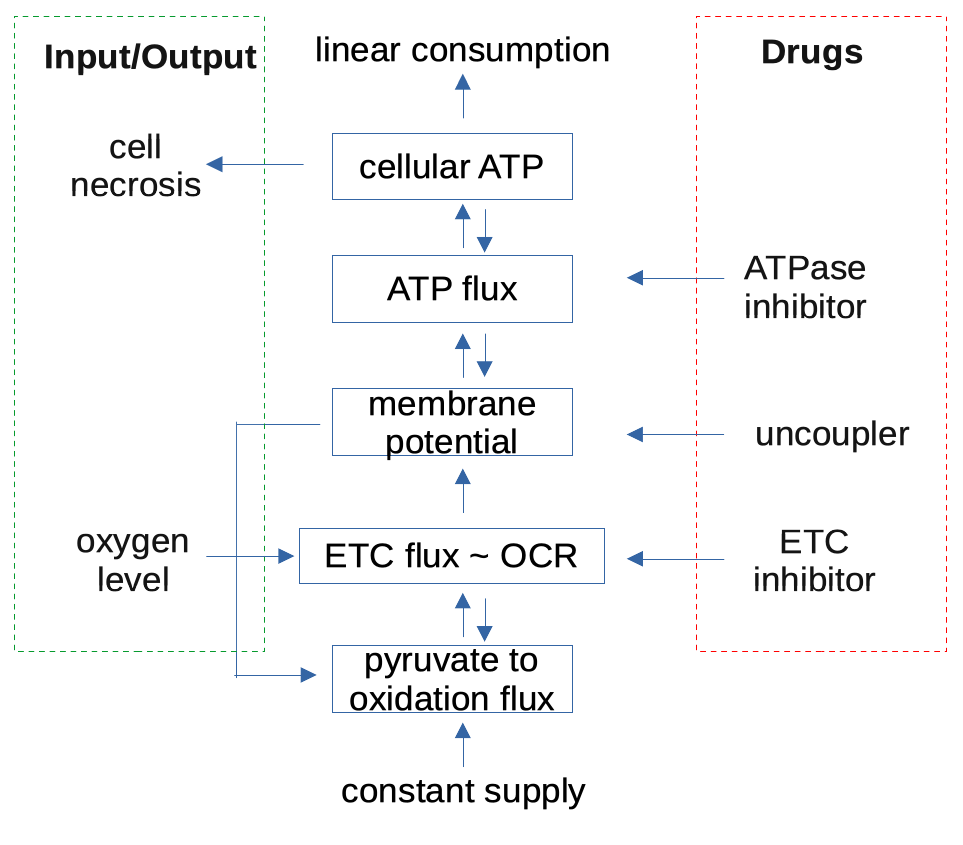
\includegraphics[width = 10cm, height = 10cm]{mito_schematic.png}
\caption{Schematic diagram of Mitochondria Submodel that illustrate Equation \ref{eq:1}. Arrows going upwards represent the movement of fluxes in the metabolic pathway, while arrows going downwards represent feedback inhibitions. In the red box are the drugs with mitochondrial toxicity, and in the green box are the input and output of Mitochondria Submodel to other submodels of SysDILI. }
\label{fig:6}
\end{figure}\\\\Figure \ref{fig:6} provides an schematic view of Equation \ref{eq:1}. Figure \ref{fig:5} shows how the submodel relates to its predecessor, MITOsym\textsuperscript{\textregistered}. The encircled variables and feedback signals remained in SysDILI. Three additional changes from MITOsym\textsuperscript{\textregistered} are summarised below.
\begin{itemize}
\item Influx to pyr2ox, the first variable of the submodel, is constant.
\item ETCF is affected by oxygen concentration, and their relation is described by Michaelis–Menten kinetics. This enables the interaction between Oxygen and Mitochondria Submodels.
\item To calculate ATPC, ATPF is multiplied by a factor of $q_5=\frac{4}{3}$ to compensate for glycolytic ATP that is not modelled (reasons and consequences in Discussion section) . 
\end{itemize}



\begin{figure}[h!]
\centering
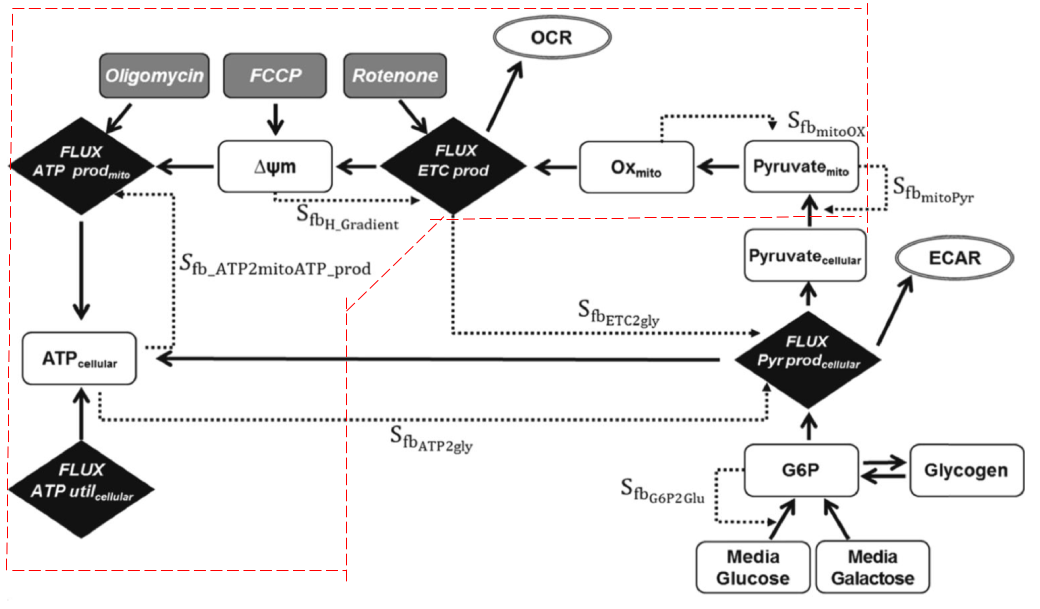
\includegraphics[width = 14cm, height = 9cm]{yang_model_modified.png}
\caption{Schematic diagram of MITOsym\textsuperscript{\textregistered} and its adaption. The encircled state variables, flux variables and feedback signals remained in SysDILI. Diagram adapted from Yang et al.\cite{y.yangMITOsymMechanisticMathematical2015} }
\label{fig:5}
\end{figure}



\myparagraph{Model Parametrisation}
Figure \ref{fig:4_1} shows how the model parameters were determined during model construction. Basal values of all variables were given in Yang et al. \{$q_1$, ... , $q_6$\} and \{$k_1$, ... , $k_6$\} were estimated, because most of the parameter values were not provided by the authors. \{$q_1$, ... , $q_6$\} were determined in such a way that the basal values of variables were ensured to be an stationary point of the ODE system. Besides $q_5$ mentioned above, $q_3$ for $\frac{d\phi}{dt}$ was calculated using physiological data (see the Methods Section). \{$k_1$, ... , $k_6$\} were fitted using the batch of drug response data provided in Yang et al., nine data sets consisting of Rotenone (ETC inhibitor), FCCP (uncoupler) and Oligomycin (ATPase inhibitor) intakes versus OCR, $\phi$, and ATPC.\begin{figure}[ht] 
  
  \begin{minipage}[b]{0.5\linewidth}
    \centering
    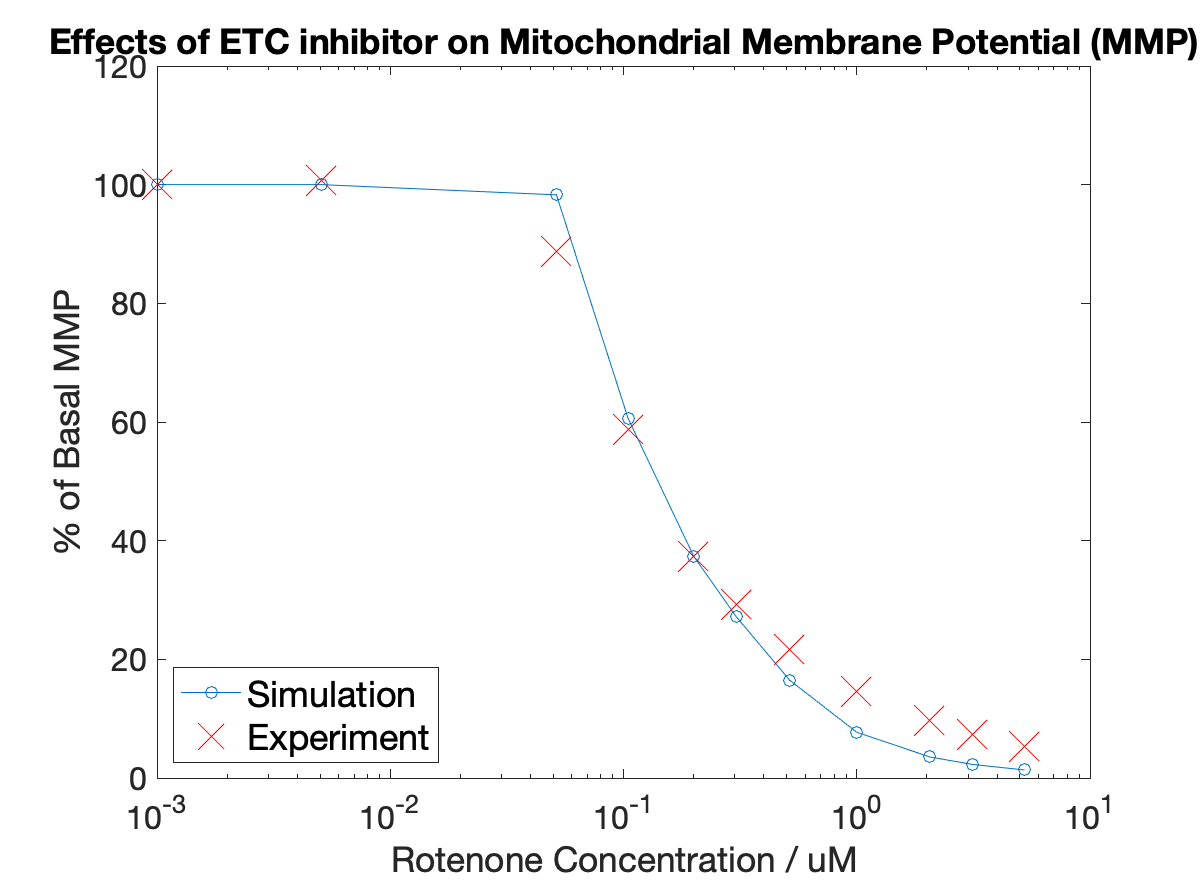
\includegraphics[width=\linewidth]{etc_mmp.png} 
  \end{minipage}%%
  \begin{minipage}[b]{0.5\linewidth}
    \centering
    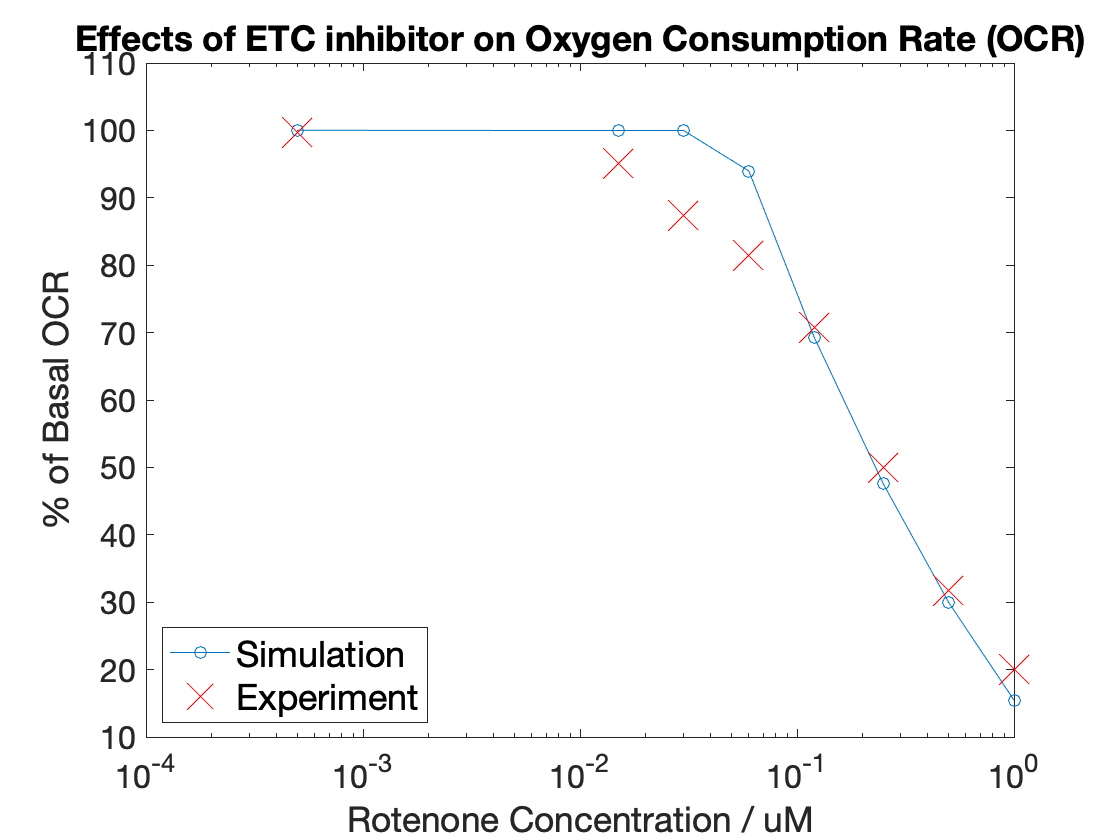
\includegraphics[width=\linewidth]{etc_ocr.png} 
  \end{minipage} 
  \begin{minipage}[b]{0.5\linewidth}
    \centering
    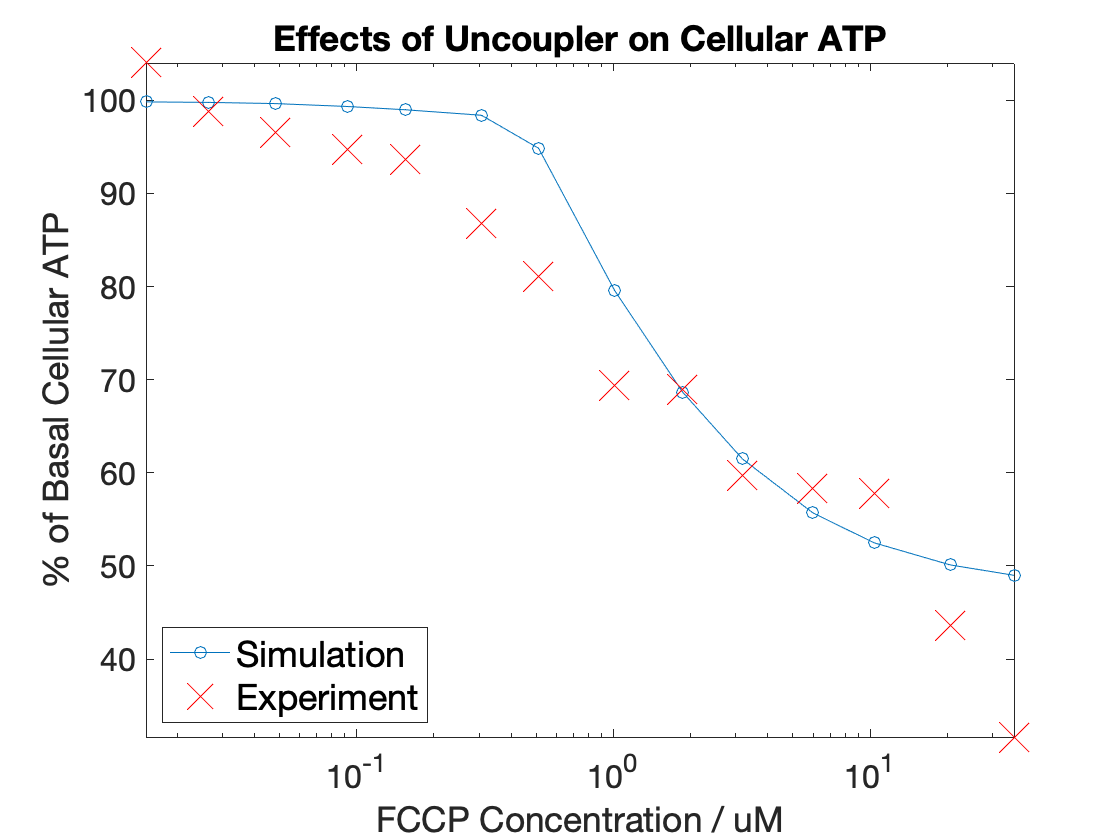
\includegraphics[width=\linewidth]{uncp_atp.png} 
  \end{minipage}%% 
  \begin{minipage}[b]{0.5\linewidth}
    \centering
    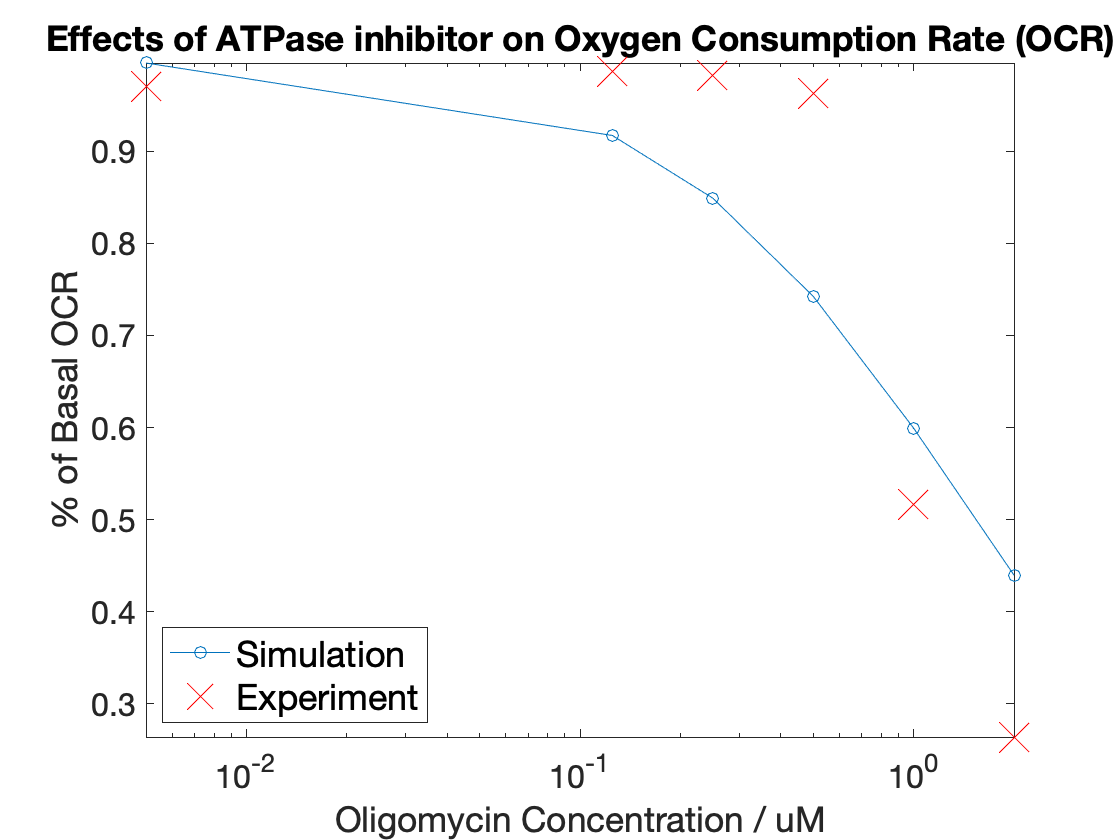
\includegraphics[width=\linewidth]{atpase_ocr.png} 
  \end{minipage} 
  \caption{Goodness-of-fit for Mitochondria Submodel in selected datasets of dose-response. Clockwise from top-left: MMP versus Rotenone, OCR versus Rotenone, OCR versus Oligomycin, cellular ATP versus FCCP. Red crosses are experimental data, and the blue line are simulated results after fitting.}
  \label{fig:quad_mito}
  \end{figure}\\\\Good fitting results of the model can be seen in Figure \ref{fig:quad_mito}. The values of parameters are listed in Method Section.
\myparagraph{Model Operation}
Figure \ref{fig:4_2} shows how the model handles unknown drugs. All parameters determined during model construction stay constant. The mechanism and the dose-response curve of the unknown drug are needed as input, then the corresponding drug-specific $km_i$ is fitted from dose-response curve, after which the simulation of this particular drug can be carried out. Alternatively, Michaelis constant (Km) can be supplied to reconstruct the dose-response curve of the unknown drug. \\\\
This procedure is different from that in Yang et al., where values of experimental Km were used directly for $km_i$ in the model \cite{y.yangMITOsymMechanisticMathematical2015}. In contrast, the submodel treats $km_i$ as nominal Km determined from experimental Km by optimisation, because the other variables might also changes with drug dose.
\begin{figure}[ht]
\begin{subfigure}{\textwidth}
\centering
    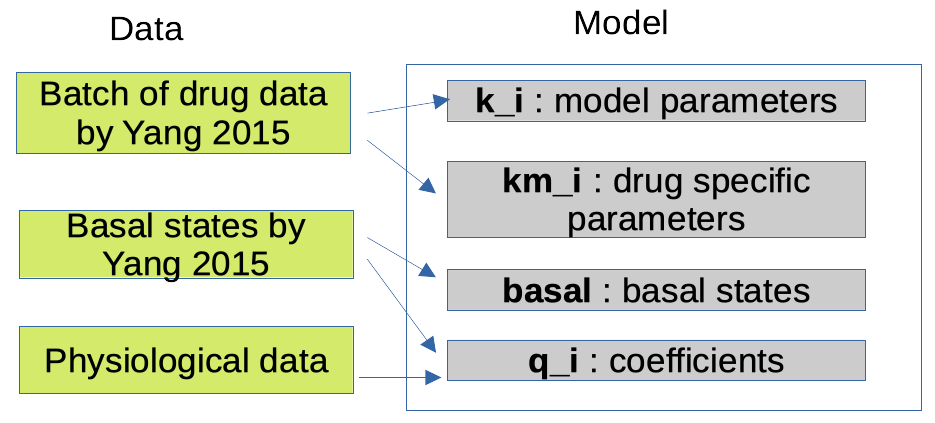
\includegraphics[width = 9cm, height = 4.5cm]{mito_step1.png}
    \caption{}
    \label{fig:4_1}
\end{subfigure}
\hfill
\begin{subfigure}{\textwidth}
\centering
    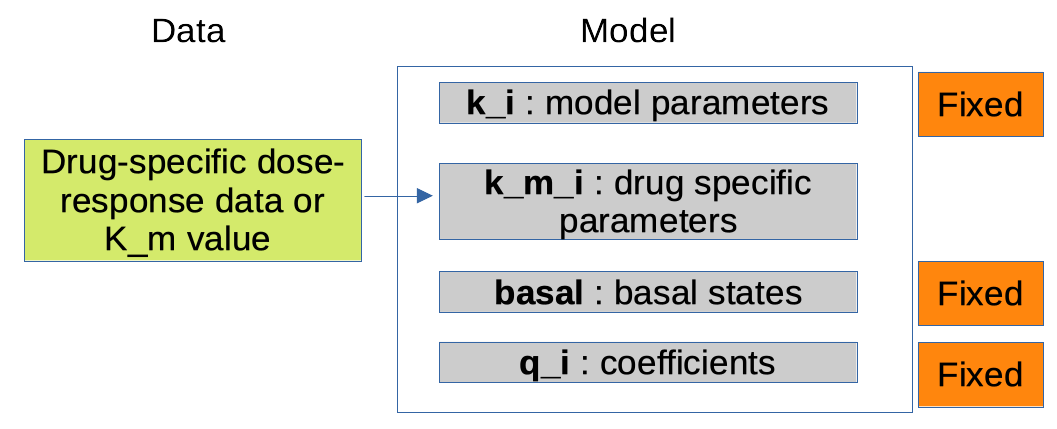
\includegraphics[width = 10cm, height = 4.5cm]{mito_step2.png}
    \caption{}
    \label{fig:4_2}
\end{subfigure}
\hfill
\caption{Schematic diagram of the parameters of Mitochondria Submodel. (a) Step One: determination of Mitochondria Submodel parameters during model construction; (b) Step Two: the operation of Mitochondria Submodel with an unknown drug, where all other parameters are fixed and the drug-specific parameters are fitted.}
\end{figure}

\subsubsection{Cell Density Submodel}
\begin{equation}\frac{d DEN}{dt}= -(k_7*\frac{{AD}^{k_9}}{{ AD}^{k_9}+{k_{8}}^{k_9}}+k_{10}*\frac{{AD}^{k_{12}}}{{ AD}^{k_{12}}+{k_{11}}^{k_{12}}})*DEN 
\label{eq:3}
\end{equation}
Equation \ref{eq:3} defines Cell Density Submodel, where DEN is the density of hepatocytes and AD is the percentage decrease of cellular ATP. Note that AD=0 when cellular ATP is above the basal level.\\\\ 
This submodel was constructed from scratch. ATP depletion is the only input variable because it is regarded as an important cause of hepatocyte death \cite{redegeldDepletionATPNot1992}. Also, ATP depletion is relatively easy to track and linked directly to mitochondrial toxicity modelled in Mitochondria Submodel. Two Hill equation terms were used, motivated by the finding that apoptosis and necrosis are both energy-dependent with ATP level as a switch between them \cite{leistIntracellularAdenosineTriphosphate1997a,tsujimotoApoptosisNecrosisIntracellular1997}.\\\\
Only acute DILI (within 12 hours) was modelled in this submodel, because it is relatively easy to model and validate with existing data. Hepatocyte regeneration is negligible within this time range, so it is not modelled and the modelled cell density is monotonically decreasing in time \cite{furchtgottModelLiverRegeneration2009}. Modelling longer term DILI might require a considerably more complex system.
\myparagraph{Model Parametrisation}
The parameters \{$k_7$, ... , $k_{12}$\} were fitted using 10 datasets of cellular ATP versus time (input) and cell viability versus time (output) from Redegeld et al. \cite{redegeldDepletionATPNot1992,redegeldInteractionCellularATP1990}. The experiments were \textit{in vitro} using rat hepatocytes, with lactate dehydrogenase (LDH) leakage as indicator for cell death, and only data from experiments with inhibition glycolytic ATP was selected (reasons in Discussion section).\\\\
Fitted results $k_7=80.5$ $min^{-1}$ and $k_{10}=0.005$ $min^{-1}$ show that the two Hill equation terms in Equation \ref{eq:3} have completely different scales, an evidence that there exist two different energy-dependent processes for cell death, namely apoptosis and necrosis. Good fitting results can be seen in Figure \ref{fig:quad_den}.
\begin{figure}[ht] 
  \begin{minipage}[b]{0.5\linewidth}
    \centering
    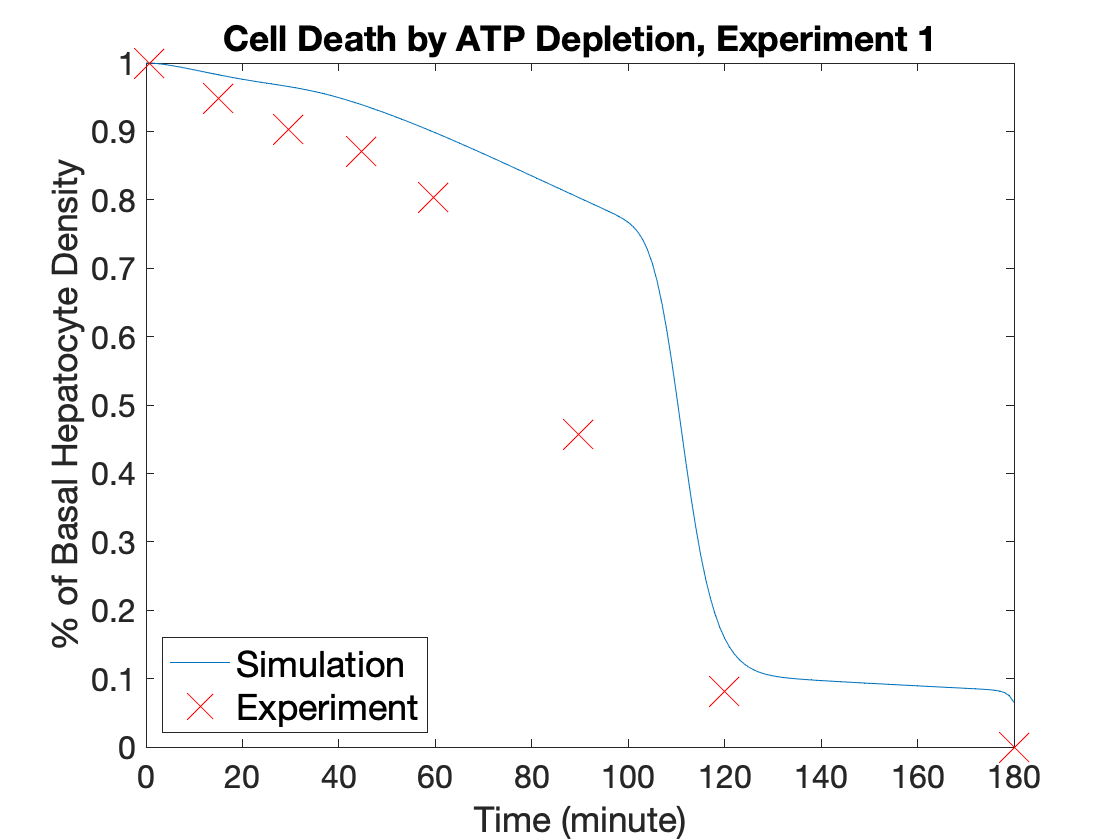
\includegraphics[width=\linewidth]{den_vali1.png} 
  \end{minipage}%%
  \begin{minipage}[b]{0.5\linewidth}
    \centering
    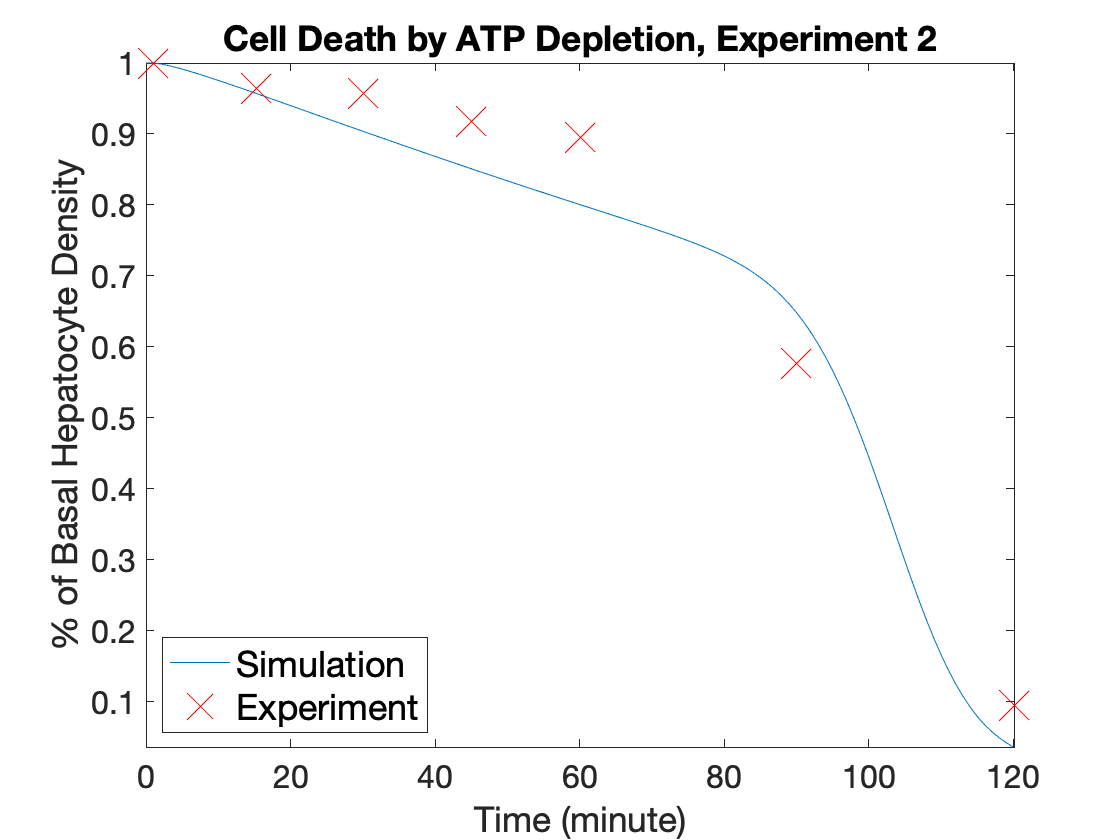
\includegraphics[width=\linewidth]{den_vali2.png} 
  \end{minipage} 
  \caption{Goodness-of-fit for Cell Density Submodel in selected datasets of cell viability versus time. The corresponding input datasets of cellular ATP versus time are not shown. Red crosses represent experimental data, and the blue line represent simulated results after fitting.}
  \label{fig:quad_den}
\end{figure}


\subsubsection{Drug Submodel}
Three options have been developed for Drug Submodel.
\begin{itemize}
    \item \textbf{Option 1: Continuous Spatiotemporal Drug Gradient}: this setup is the same as Oxygen Submodel except an extra permeability coefficient when drug crosses cell membrane, modelled by changing the PDE at the sinusoid-hepatocyte interface to the following \cite{leedaleMultiscaleModellingDrug2020}.
    \begin{equation}
        D_s*\frac{\partial C_s}{\partial r}=D_h*\frac{\partial C_h}{\partial r}=Q(C_s-C_h)
        \label{eq:drug}
    \end{equation}
    In Equation \ref{eq:drug}, Q is the drug-specific permeability coefficient. $D_s$ and $D_h$ are diffusion coefficients of drug in sinusoid and hepatocytes, respectively. $C_s$ and $C_h$ are the drug concentration in sinusoid and hepatocytes, respectively. In the numerical algorithm, this difference was modelled by increasing the interface from one unit to two to accommodate the extra condition $Q(C_s-C_h)$.\\\\Figure \ref{fig:quad_drug} shows the output of drugs with high and low permeability. High permeability results in a radial gradient of drug concentration, while concentration discontinuity can be seen across the interface for drug with low permeability, as one would expected.
     \begin{figure}
 \begin{minipage}[b]{0.5\linewidth}
    \centering
    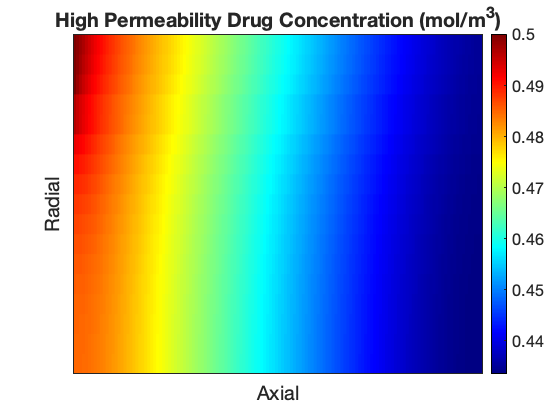
\includegraphics[width=\linewidth]{drug_high.png} 
  \end{minipage}%%
  \begin{minipage}[b]{0.5\linewidth}
    \centering
    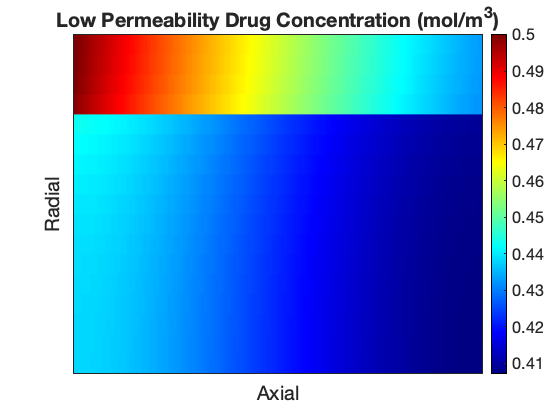
\includegraphics[width=\linewidth]{drug_low.png} 
  \end{minipage} 
  \caption{Output of Drug Submodel Option 1. The axes and layout are the same as those illustrated in Figure \ref{fig:oxy} of Oxygen Submodel. Q=4.8948 $\mu m/s$ and 0.0081 $\mu m/s$ were used to represent drugs with high and low permeability, respectively \cite{leedaleMultiscaleModellingDrug2020}. Drug gradients with different permeabilities were created as expected: high permeability leads to continuous gradient, while low permeability results in discontinuity at the interface.}
  \label{fig:quad_drug}
\end{figure}
    \item \textbf{Option 2: Two-Compartment Model}: no drug gradient, only two compartments: sinusoid (central) and hepatocytes (peripheral). In Equation \ref{eq:two_comp}, $k_{sh}$, $k_{hs}$, $k_e$ and $k_{metabolism}$ stand for first-order rate constants for drug distribution, redistribution, elimination and metabolism, respectively. I is the rate of drug input which may vary with time.\\ 
    \begin{equation}
    \begin{aligned}
        &\frac{d C_s}{dt}=-(k_{e}+k_{sh})*C_s+k_{hs}*C_h+I \\
        &\frac{d C_h}{dt}=-(k_{m}+k_{hs})*C_h+k_{sh}*C_s \\
        \end{aligned}
        \label{eq:two_comp}
    \end{equation}
    \begin{figure}[h!]
\centering
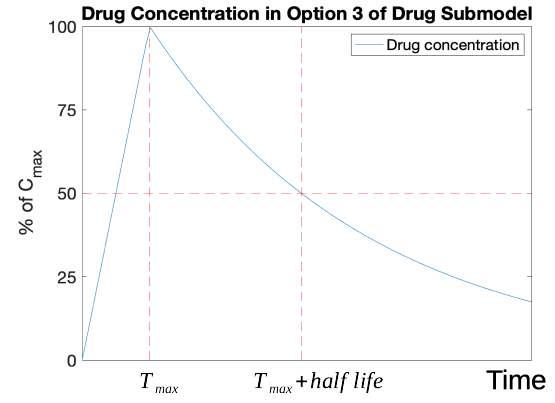
\includegraphics[width = 10cm, height = 8cm]{dr_sketch.png}
\caption{Illustration of drug concentration over time in Option 3 of Drug Submodel. Drug concentration increases linearly and reaches $C_{max}$ at time $T_{max}$ before decreasing exponentially with fixed half life.}
\label{fig:dr_sketch}
\end{figure}
    \item \textbf{Option 3: One-Compartment Model}: hepatocytes domain is the only compartment. Drug concentration increases linear to reach $C_{max}$ after time $T_{max}$, and then drops exponentially with a fixed half life, as illustrated in Figure \ref{fig:dr_sketch}.\end{itemize}
Option 1 is more compatible with the theme of SysDILI, but it is difficult to validate in the context of human liver. Option 2 and 3 are pharmacokinetics model, so they might be more reliable and easier to parametrise with existing data. Option 3 was selected for the subsequent simulations, because human pharmacokinetics data of $C_{max}$, $T_{max}$ and half life of drugs are readily available, which makes Option 3 easier to manipulate and track, allowing fair comparisons of different drugs. Option 1 and 2 might be used later in \textit{in vitro} scenarios where measurement and manipulation are easier.

\subsection{Toxicity Simulations}
As said in Introduction section, submodels can be freely assembled for simulation. A few different combinations with increasing complexity have been tried. The mechanism of ETC inhibition was selected for simulations. Drugs and doses used in simulations are summarised in Table \ref{tab:drug}. Drug Submodel Option 3 was used with $T_{max}=2$ hours and half life of 4.5 hours.
\begin{table}
\centering
\begin{tabular}{|c|c| c| c| c |} 
 \hline
 \textbf{Trial IDs} & \textbf{Drug Names} & \textbf{$k_m$} & \textbf{Dose ($C_{max}$)} & \textbf{Known Toxicity}\\
 \hline\hline
A &Aripiprazole & 0.75 & 0.1 & 0 \\
\hline
B &Aripiprazole & 0.75 & 0.2 & 0 \\
\hline
C &Known Drug & 2.7 & 1.3 & 0.5 \\
\hline
D &Known Drug & 2.7 & 5 &  1\\
\hline
E &Control & 0.35 & 1.3 & 1 \\
\hline
F& Control & 0.35 & 5 &  1\\
\hline

\end{tabular}
\caption{Drugs and doses in the simulations. Toxicity value of 0 means safe, 1 means toxic and 0.5 means moderately toxic.}
\label{tab:drug}
\end{table}
\subsubsection{Drug+Mitochondria (DM)}
\begin{figure}[h!]
\centering
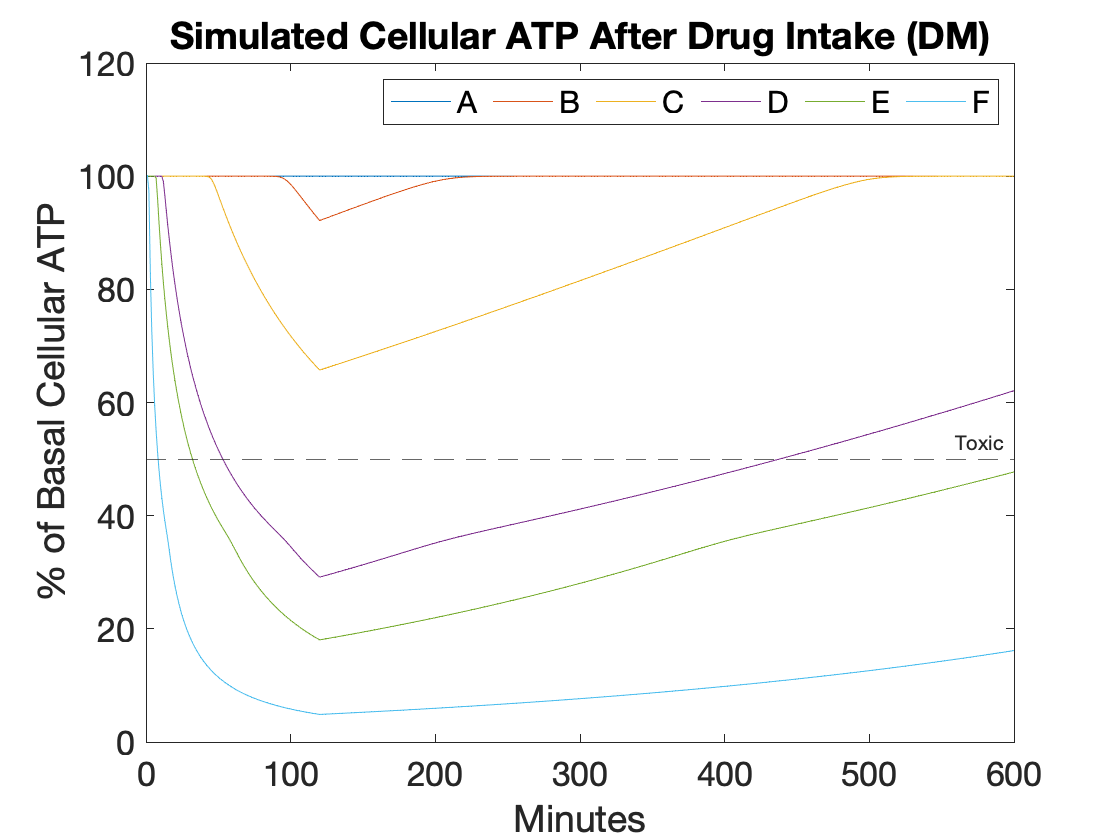
\includegraphics[width = 12cm, height =10cm]{dm.png}
\caption{Toxicity simulation outcome of DM model. Trial A and B shows very limited change in cellular ATP, implying safety. Cellular ATP of Trial D, E and F drop below toxicity criterion for a significant period, which agrees with their known toxicity. Trial C appears to be safe.}
\label{fig:dm}
\end{figure}
When Cell Density Submodel is not involved, cellular ATP level is used as surrogate. Cellular ATP lower than 50 percent of basal level implies toxicity, because it marks the onset of immune mediated induced necrosis by TNF-$\alpha$ \cite{leistIntracellularAdenosineTriphosphate1997a,nieminenATPDepletionRather1994a,cannonEffectsFructoseAdenosine1991}. No spatial gradient is involved in DM model, so oxygen concentration was fixed to the basal level in Mitochondria Submodel.\\\\
Figure \ref{fig:dm} shows the outcome. Trial D, E and F were correctly predicted to be toxic, while Trial A and B were correctly predicted to be safe with almost no change to cellular ATP levels. However, Trial C was predicted to be safe, which is questionable. Further simulation and investigation are necessary.
\subsubsection{Drug+Mitochondria+Oxygen (DMO)}
\begin{figure}[h!]
\centering
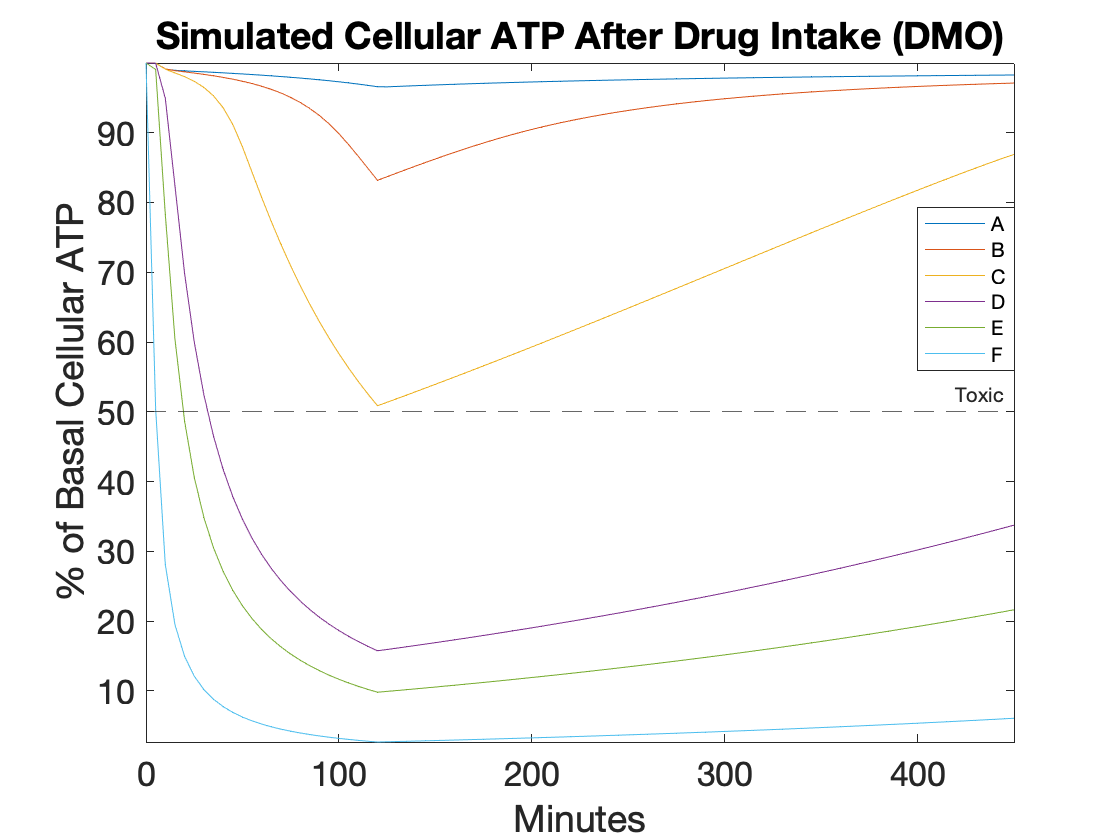
\includegraphics[width = 12cm, height =10cm]{dmo.png}
\caption{Toxicity simulation outcome of DMO model. Cellular ATP level is the average of the entire hepatocytes domain. The outcome is similar to that of DM model in Figure \ref{fig:dm}, with result of Trial C correctly showing its mild toxicity.}
\label{fig:dmo}
\end{figure}
Spatial gradients appeared after adding Oxygen Submodel. When assembling submodels, the spatially discretised domain setup of Oxygen Submodel was used, while each discretised point received an independent copy of ODE-based Mitochondria Submodel and Drug Submodel.\\\\
In the numerical simulation, equations of Oxygen and Mitochondria Submodels were not fused together into a larger PDE system, because the convergence of oxygen PDE system is much faster than the time step chosen for Mitochondria ODE system, 1 minute. Therefore, at the start of each time step, with OCR given by Mitochondria Submodel, Oxygen Submodel was run until convergence, producing an oxygen gradient for Mitochondria Submodel to use in the next time step.\\\\
Adding the oxygen gradient has rendered a more realistic result for Trial C, as shown in Figure \ref{fig:dmo}.
\subsubsection{Drug+Mitochondria+Oxygen+Density (DMOD)}
\begin{figure}[h!]
\centering
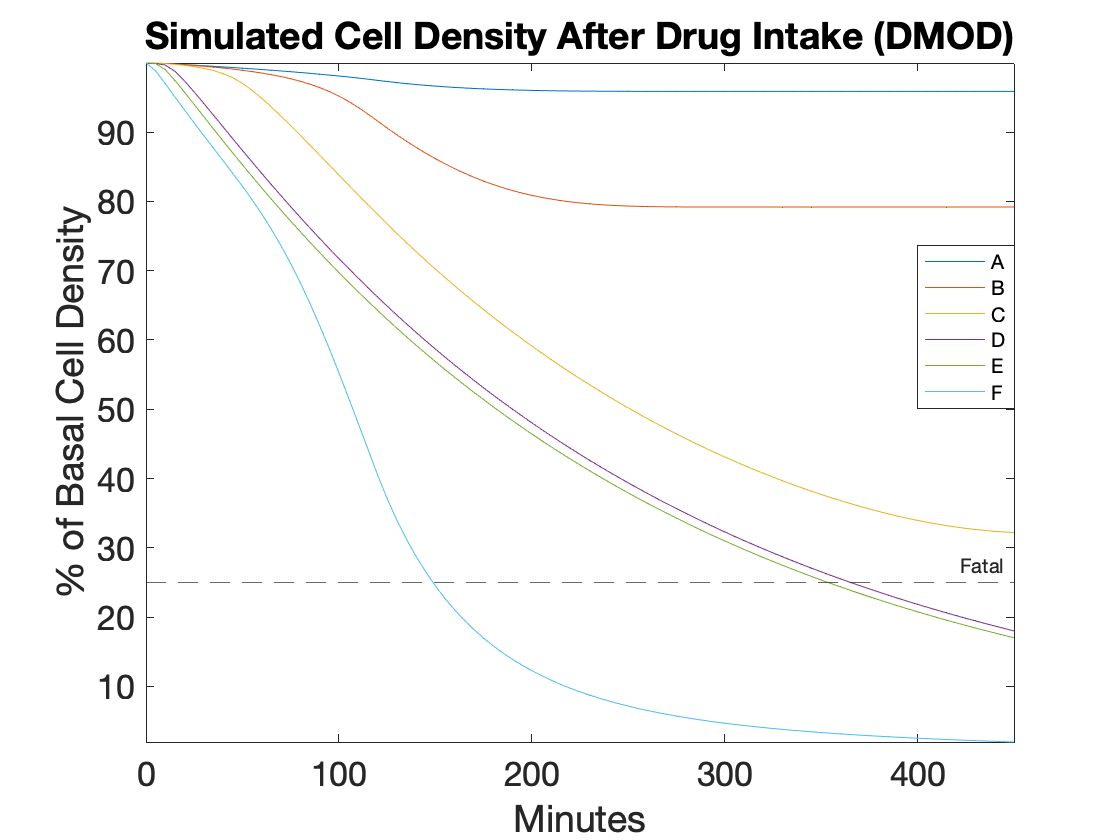
\includegraphics[width = 12cm, height =10cm]{dmod.png}
\caption{Toxicity simulation outcome of DMOD model. Cell density level is the average of the entire hepatocytes domain. The toxicity predictions are similar to those in DMO model in Figure \ref{fig:dmo}.}
\label{fig:dmod}
\end{figure}



\begin{figure}[h!]
\centering
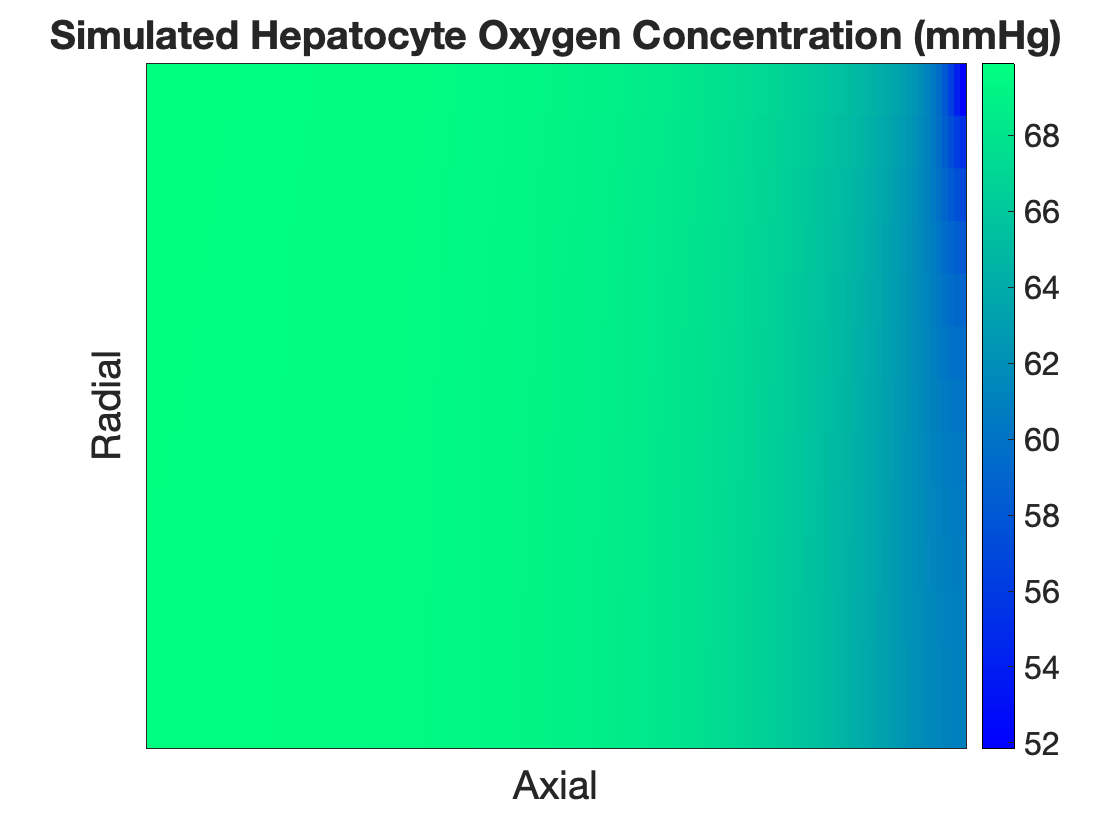
\includegraphics[width = 9cm, height =7cm]{loss.png}
    \caption{Hepatocyte Oxygen Concentration of Trial F in DMOD model after 450 minutes. Oxygen gradient is mostly lost when large dose of drug with mitochondrial toxicity causes severe DILI.}
\label{fig:loss}
\end{figure}
\begin{figure}[h!]
\centering
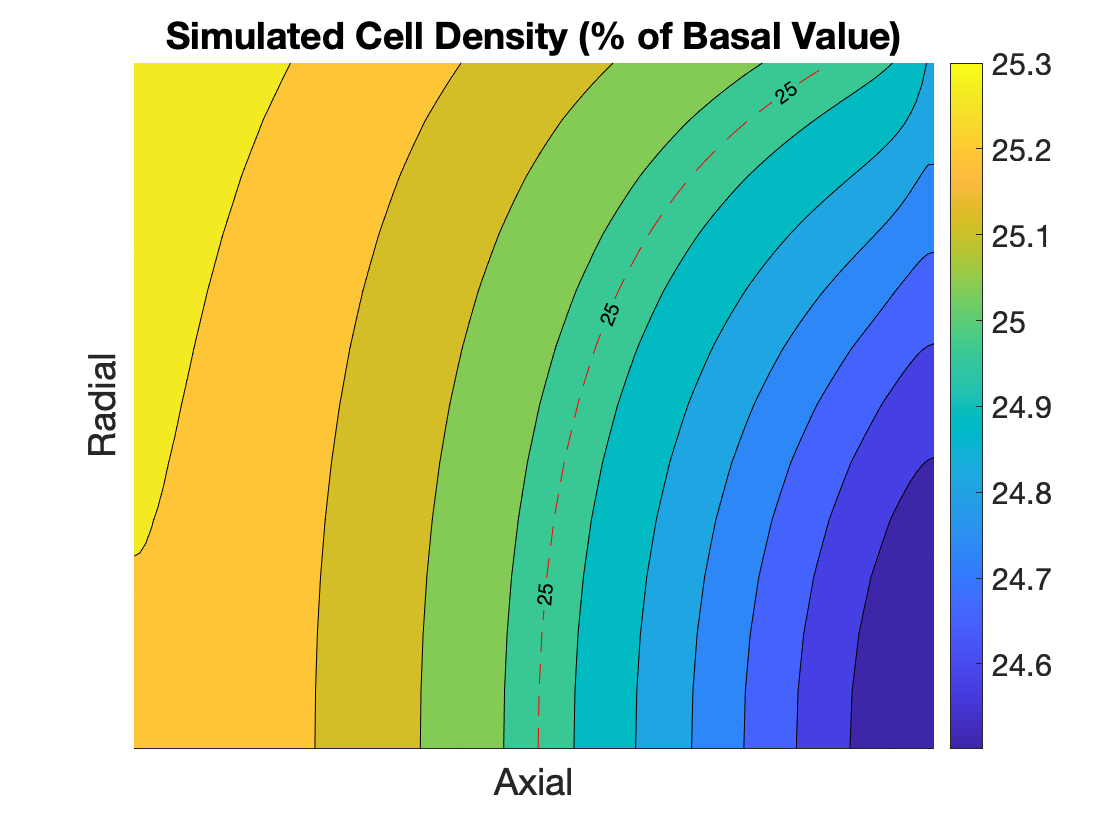
\includegraphics[width = 11cm, height =9cm]{gradient.png}
    \caption{Cell Density of Trial D in DMOD model after 365 minutes. 25 percent marked with red dash line. Cell density is the lowest in zone 3, which indicates its relative vulnerability to DILI.}
    \label{fig:gradient}
\end{figure}

After adding Cell Density Submodel, cellular ATP is no longer needed as surrogate. Cell density below 25 percent of basal value is considered fatal damage \cite{furchtgottModelLiverRegeneration2009}.\\\\
Figure \ref{fig:dmod} shows the outcome of DMOD model. Trial D, E and F are confirmed to be fatally toxic, while Trial C is close to the borderline as expected. Apart from average values, simulated spatial gradients also contain useful insights. Research suggests that metabolic zonation of liver is often lost in liver diseases \cite{kietzmannMetabolicZonationLiver2017a}, as confirmed in Figure \ref{fig:loss}. When compared to Figure \ref{fig:quad}, simulated outcome of Trial F by DMOD model indicates that severe DILI damages the oxygen gradient. Figure \ref{fig:gradient} shows the simulated spatial distribution of cell density of Trial D, which indicates that zone 3 is relatively vulnerable to mitochondrial DILI, especially the part furthest away from hepatic sinusoid.
 %The simulations confirm the importance of spatial distribution
%50 percent ATP is the switch! test density model compare to one single Hill equation
\section{Discussion}
The submodels of SysDILI have been developed independently. However, significant effort was made to ensure that the submodels
work smoothly together and validate each other. Holistic approach of systems biology was used to study interactions quantitatively through PDEs and ODEs, allowing SysDILI to go beyond the reductionist approach of investigating each underlying process while fixing the others \cite{tavassolySystemsBiologyPrimer2018}. \\\\
While some of the methods and models in SysDILI build on previous research, several new original advances have been incorporated in the presented analyses:
\begin{itemize}
    \item Oxygen transport by haemoglobin was modelled dynamically, with the rebalancing process at the end of time step.
    \item {$km_i$} for the drugs in Mitochondrial Submodel were treated as nominal values and determined by optimisation, to handle the complexity of model.
    \item Two Hill equation terms were used in Cell Density Submodel to capture the combined effects of energy-dependent apoptosis and necrosis, instead of a separate model for each process. This "guided" black box model balances effectiveness and simplicity.
\end{itemize}
\subsection{Model Design}
SysDILI currently focuses on mitochondrial toxicity for two reasons. Firstly, mitochondria activities are relatively easy to measure and bioenergetics is well characterised. Secondly, mitochondria interacts well with other submodels. as shown in Figure \ref{fig:1}, it is directly associated with respiration and oxygen gradient, as well as cell death by ATP depletion.\\\\
Instead of designating artificial zones or gradients, SysDILI was engineered to create the gradients by constructions to investigate the root cause. Liver zonation is an observed result of various gradients that regulate it. There is evidence that liver zonation is rather dynamic and not static, changing with the gradients \cite{kietzmannMetabolicZonationLiver2017a}. Meanwhile, artificial gradients such as oxygen gradient was used to investigate its effects \cite{kangMetabolicPatterningChip2018}. Acknowledging their effects, it is possible to go even deeper and uncover the cause of substance gradients, such as production, consumption and transport.\\\\
In Mitochondria Submodel, mitochondrial ATP was multiplied by a factor $q_5$ to account for glycolytic ATP. This might underestimate  cellular ATP level when mitochondria activity gets inhibited, because glycolytic ATP production can alternatively be sustained by anaerobic glycolysis temporarily \cite{harrisEnergyMetabolismGlycolysis2019}. Another option is to fix glycolytic ATP at the basal value, but this instead overestimates cellular ATP, because sustained anaerobic analysis leads to the build-up of lactic acid, which eventually causes life-threatening lactic acidosis \cite{harrisEnergyMetabolismGlycolysis2019}. The treatment of glycolytic ATP that underestimates cellular ATP and hence drug safety was chosen, because it is conventional to have a conservative estimate for safety concern. Moreover, short term cell death in SysDILI might correspond to significant human DILI in longer term.\\\\
More importantly, hepatocyte viability is more sensitive to depletion of glycolytic ATP than mitochondrial ATP \cite{redegeldDepletionATPNot1992}. Redegeld et al. suggests that this might be due to the sub-cellular distribution of ATP: glycolytic ATP in the vicinity of cell membrane is more available to the ATP-driven processes at the membrane, which is the limiting factor in cell death \cite{jonesIntracellularDiffusionGradients1986}. For example, the calcium pump of cell membrane in pancreatic cancer cell can be sustained by glycolytic ATP, and the cell survives without mitochondrial ATP \cite{jamesGlycolyticATPFuels2013a}. Therefore, to parameterise Cell Density Model, only experiments with glycolysis inhibition were used, which again leads to underestimation of drug safety as expected.
%\subsection{Findings}
\subsection{Limitations and Potential Improvements}
The focus of the project was on model construction and validation. Further research would be done to explore SysDILI and gain insight into drug-liver interactions, which was outside the scope of this research due to time restriction.\\\\
SysDILI relies on published data, which tend not to be ideal. The datasets used to parameterise each submodel are inconsistent. Parameters of HepaRG normal human hepatocyte were used in Oxygen Submodel, while all data used in Mitochondria Submodel is from HepG2 human liver cancer cell with lower metabolic activities than normal hepatocytes \cite{vinkenProtocolsVitroHepatocyte2015}. Cell Density Submodel were fitted with rat hepatocyte in \textit{in vitro} setting. Therefore, despite each submodel being quantitative, at this stage SysDILI should be regarded as qualitative instead of quantitative model. The assumption is that the data inconsistency does not change the qualitative outcome.\\\\
Mitochondria Submodel can be upgraded to Bioenergetics Submodel by implementing the entire MITOsym and improving it \textsuperscript{\textregistered}. Variables of glycolytic ATP, lactate, glucose and glycogen will be available, after which toxicity mechanisms affecting glycolysis and glycogenolysis can be studied. Glycolytic ATP and mitochondrial ATP can be treated separately to eliminate the bias in Cell Density Submodel, the underestimation of drug safety mentioned above. Data from galactose-grown hepatocytes might be useful to isolate the effect of mitochondrial ATP, because galactose glycolysis yields no net ATP \cite{dykensMitochondrialToxicity2014b,shiratoriGlycolyticSuppressionDramatically2019}. A model of lactate might be introduced, because as an end product it might inhibit anaerobic glycolysis that sustains ATP production under mitochondrial dysfunction. It can potentially become a new stand-alone submodel of SysDILI, because liver is particularly important in lactate metabolism, accounting for 60 percent of lactate clearance through Cori cycle \cite{levyLactateShockState2006,harrisEnergyMetabolismGluconeogenesis2021} .\\\\
Mitochondria Submodel might also be used to infer the toxicity mechanism of an unknown drug. Given drug-response data of different variables, all {$km_i$} can be determined together through optimisation. The smaller $km_i$ may indicate a bigger effect through that particular mechanism.\\\\With lots of parameters in Mitochondria Submodel, a sensitivity analysis similar to that in Section \ref{section:sens} can benefit the understanding of the complicated interactions and identify the significant parameters for further investigation.\\\\
As mentioned before, Cell Density Submodel only models short term DILI within 12 hours for simplicity. It might be extended to model longer term DILI, with a more complex and mechanistic ODE system modelling mechanisms and regulatory pathways for regeneration, apoptosis and necrosis \cite{furchtgottModelLiverRegeneration2009,remienMathematicalModelingLiver2012}. Data from \textit{in vitro} experiment of rat hepatocyte LDH might be replaced by \textit{in vivo} measurement of Alanine transaminase (ALT), a commonly used indicator specific to human DILI \cite{gianniniLiverEnzymeAlteration2005,watkinsDrugSafetySciences2011a}.\\\\
For Drug Submodel, more drugs with known $T_{max}$ and half life can be simulated, instead of fixing these values. With more information of drug metabolic rates and mechanisms, Option 1 can be used to simulate MPS, where the intake of drug is easier to control than in \textit{in vivo} scenarios.\\\\
The domain setup to model human liver can be improved by adding space of Disse. More molecules that are significant in liver zonation such as glucose and growth factors can be added, using models similar to Oxygen or Drug Submodel \cite{kietzmannMetabolicZonationLiver2017a}.\\\\Domains and submodels can be easily changed or added to adapt to the setting of a particular MPS. Resources can be saved by narrowing down the range of drug dose for MPS experiments, using the toxicity predictions from SysDILI.\\\\
As for implementation, MATLAB codes might be made more organised using MATLAB SimBiology toolbox, which takes care of variables and their units and streamlines model analysis. If large scale simulation is needed, the core program of SysDILI can be translated into Python.
\section{Methods}
All simulations, optimisations and visualisation were performed in MATLAB. The ODE systems for mitochondria, cell density and drug were solved numerically using ODE15s solver. The PDE systems (convection–diffusion-reaction equation) for oxygen and drug were solved by a numerical solver developed from scratch, using Crank-Nicolson method for diffusion, the upwind scheme for convection and Euler method for reaction. Parameters fitting for mitochondria and cell density were performed using multi-start global optimisation algorithm with interior-point method as the local optimiser available in MATLAB. For the rebalancing of haemoglobin and plasma oxygen, Equation \ref{eqn:reba} was solved by a Newton–Raphson method root finder developed from scratch to speed up simulations. Convergence was used as stopping criteria for the numerical simulations: $\frac{||M_{n+1}-M_n||}{\Delta t}<\epsilon$, where $M_n$ is the matrix of variable at $n$-th time step. MATLAB Global Sensitivity Analysis Toolbox was used in FAST sensitivity analysis.
\begin{table}
\centering
\begin{tabular}{|c | c| c|} 
 \hline
 \textbf{Parameters} & \textbf{Values} & \textbf{Sources}\\
 \hline\hline
 Sinusoid Length & 275 $\mu$m & Ehrlich et al. \cite{ehrlichChallengesOpportunitiesDesign2019}\\ 
 \hline
Sinusoid Diameter & 10-15 $\mu$m (12.5 $\mu$m) & Maynard et al. \cite{maynardChapter14Liver2019}\\
\hline
Hepatocyte Diameter & 25-30 $\mu$m (27.5 $\mu$m) & Meyer et al. \cite{meyerChapterLiver2016}\\
\hline
$v$, Sinusoid Blood Flow Velocity & 300-650 $\mu$m/s (400 $\mu$m/s) & Muller et al.\cite{mullerEstimatingBloodFlow2009}\\
\hline
$v_{max}$ of hepatocyte OCR & 44 $\mu$M/s & Leedale et al. \cite{leedaleMultiscaleModellingDrug2020}\\
\hline
$k_m$ of hepatocyte OCR & 6.24 $\mu$M & Leedale et al. \cite{leedaleMultiscaleModellingDrug2020}\\
\hline
$O_2$ Diffusion Coefficient in Plasma & 2180 $\mu m^2$/s & Goldstick et al. \cite{goldstickDiffusionOxygenPlasma1976}\\
\hline
 $O_2$ Diffusion Coefficient in Hepatocytes & 1600 $\mu m^2$/s & Leedale et al. \cite{leedaleMultiscaleModellingDrug2020}\\
\hline

\end{tabular}
\caption{Human Physiological Parameters for Oxygen Submodel}
\label{Tab:2}
\end{table}
\\\\Table \ref{Tab:2} lists parameters in Oxygen Submodel from human physiological data. Time ($\Delta t=4.5*10^{-3}s$) and space ($\Delta x=2 \mu m$) steps were chosen to satisfy the stability conditions of Crank-Nicolson method and the upwind scheme.
Throughout Oxygen Submodel partial pressure with unit mmHg were used in place of concentration, because they are directly proportion by Henry's law
with solubility coefficient of oxygen in plasma $\alpha=3\times10^{-5}$ml $O_2$/ml plasma/mmHg \cite{pittmanOxygenTransport2011}.\\\\
For the boundary conditions of Oxygen Submodel (Figure \ref{fig:oxy}), zero flux Neumann boundary condition was chosen for the boundary of hepatocytes domain. At the sinusoid entrance, plasma oxygen was given Dirichlet boundary condition as mentioned above while plasma and haemoglobin oxygen are in equilibrium. At the sinusiod exit, both plasma and haemoglobin oxygen have convection only, the diffusion of plasma oxygen at the exit is negligible.\\\\


\begin{table}[]
    \centering
\begin{tabular}{|c | c| c|c|} 
 \hline
 \textbf{Parameters} & \textbf{Values} &\textbf{Methods}& \textbf{Sources}\\
 \hline\hline
 $k_1$ & 0.993 V  & Optimisation & Yang et al. \cite{y.yangMITOsymMechanisticMathematical2015}\\ 
\hline
 $k_2$ & 67  & Optimisation & Yang et al. \cite{y.yangMITOsymMechanisticMathematical2015}\\ 
\hline
 $k_3$ & 0.0372 mM  & Optimisation & Yang et al. \cite{y.yangMITOsymMechanisticMathematical2015}\\ 
\hline
 $k_4$ & 32.4  & Optimisation & Yang et al. \cite{y.yangMITOsymMechanisticMathematical2015}\\ 
\hline
 $k_5$ & 6787 mM $min^{-1}$ $V^{-1}$  & Optimisation & Yang et al. \cite{y.yangMITOsymMechanisticMathematical2015}\\ 
\hline
 $k_6$ & 18971 $min^{-1}$ & Optimisation & Yang et al. \cite{y.yangMITOsymMechanisticMathematical2015}\\ 
\hline
 $k_7$ & 80.5 $min^{-1}$  & Optimisation & Redegeld et al. \cite{redegeldDepletionATPNot1992,redegeldInteractionCellularATP1990}\\ 
\hline
 $k_8$ & 1.07  & Optimisation & Redegeld et al. \cite{redegeldDepletionATPNot1992,redegeldInteractionCellularATP1990}\\ 
\hline
 $k_9$ & 88.6  & Optimisation & Redegeld et al. \cite{redegeldDepletionATPNot1992,redegeldInteractionCellularATP1990}\\ 
\hline
 $k_{10}$ & 0.005 $min^{-1}$ & Optimisation & Redegeld et al. \cite{redegeldDepletionATPNot1992,redegeldInteractionCellularATP1990}\\ 
\hline
 $k_{11}$ & 0.167  & Optimisation & Redegeld et al. \cite{redegeldDepletionATPNot1992,redegeldInteractionCellularATP1990}\\ 
\hline
 $k_{12}$ & 0.877 & Optimisation & Redegeld et al. \cite{redegeldDepletionATPNot1992,redegeldInteractionCellularATP1990}\\ 
\hline
 $q_1$ & 46 mmHg $mM^{-1}$ min  & Assumption/Basal & Yang et al. \cite{y.yangMITOsymMechanisticMathematical2015}\\
\hline
 $q_2$ & 331 V $mM^{-1}$  & Basal & Yang et al. \cite{y.yangMITOsymMechanisticMathematical2015}\\
\hline
 $q_3$ & 0.199 V $pmol^{-1}$ & Estimation/Calculation & see Methods Section\\
\hline
 $q_4$ & 0.999 V   & Basal& Yang et al. \cite{y.yangMITOsymMechanisticMathematical2015}\\
\hline
 $q_5$ & $\frac{4}{3}$   & Assumption & see Results Section\\
\hline
 $q_6$ & 3.70 $mM^{-1}$  & Basal & Yang et al. \cite{y.yangMITOsymMechanisticMathematical2015}\\
\hline
\end{tabular}
\caption{Parameters for Mitochondria Submodel and Cell Density Submodel. Methods of "Basal" means ensuring that basal values form a stationary point (see Results Section).}
\label{Tab:para}
\end{table}
\begin{equation}
\begin{aligned}
\Delta \phi&=\frac{RT}{nF}*ln(\frac{[H^+]_{out}}{[H^+]_{in}})\\
\frac{d \Delta \phi}{dt}&=\frac{RT}{nF}*(\frac{1}{[H^+]_{out}}*\frac{d [H^+]_{out}}{dt}-\frac{1}{[H^+]_{in}}*\frac{d [H^+]_{in}}{dt})\\
&=\frac{RT}{nF}*(\frac{1}{[H^+]_{out}}+\frac{1}{[H^+]_{in}})*\frac{d ATP}{dt}*k_{[H+]/ATP}\\
&=\frac{RT}{nF}*(\frac{1}{10^{pH_{out}}}+\frac{1}{10^{pH_{in}}})*\frac{d ATP}{dt}*k_{[H+]/ATP}\\
\frac{d \Delta \phi}{d ATP}&=\frac{RT}{nF}*(\frac{1}{10^{pH_{out}}}+\frac{1}{10^{pH_{in}}})*k_{[H+]/ATP}\\
    \end{aligned}
    \label{eq:mmp}
\end{equation}\\\\
Table \ref{Tab:para} lists the values of all parameters in Mitochondria and Cell Density Submodels. $q_3$, the change to MMP potential per unit of ATP produced, was calculated using physiological values. Nernst potential was differentiated to calculate this constant, as shown in Equation \ref{eq:mmp} \cite{zorovaMitochondrialMembranePotential2018}. $k_{[H+]/ATP}=3$, because 3 protons are moved out to produce 1 ATP \cite{brandATPRatioATP1977}. pH values of the mitochondrial matrix and the inter-membrane space are $pH_{in}=7.78$ and $pH_{out}=6.88$, respectively \cite{porcelliPHDifferenceOuter2005}.
\pagebreak
\section*{Acknowledgements}
Firstly, I wish to thank my supervisor Dr Di Veroli, who gave me the chance to participate in this project and work with the colleagues from the world-class pharmaceutical company AstraZenca. I really appreciate the concise and spot-on feedbacks that he gave me. He challenged me to question every assumption that I made. He also set high standards for my presentation, which I am now aware is very important in biological science. I will keep the meticulous attitude towards science and always pursue excellence in my future research.\\\\
I also wish to thank Dr Uatay, my day-to-day supervisor. Without all the basic material that he provided, it would have been impossible for me to start this project. When I faced the "crossroads", he was always ready to give me guidance. Despite my inexperience in modelling and scientific research in general, he was patient enough to explain the basic knowledge and principles to me. With his expertise in both quantitative methods and liver physiology, he is a good inspiration for my personal development.\\\\
I am also grateful to all the course organisers and administrators of Part III Systems Biology. They have made it possible for me, a mathematics student who did not even study A-Level Biology, to kick start my research in biological science. More importantly, with all the affirmative experience and support from this course, now I am confident and passionate to embark on this wonderful journey in scientific research.
\pagebreak



\bibliographystyle{plain}
\bibliography{thesis}

\end{document}